\chapter{Negative Pion Cross Section Measurement}\label{ch:PionXS}
{\raggedleft ``\emph{Y ella es flama que se eleva, Y es un p\'ajaro a volar.} \par}
{\raggedleft \emph{En la noche que se incendia, estrella de oscuridad}\par}
{\raggedleft \emph{que busca entre la tiniebla, la dulce hoguera del beso.}"\par}
{\raggedleft -- Lila Downs,   2002 -- \par}%Benediction And Dream,
\vspace{0.5cm}

In this chapter, we show the result of the thin slice method to measure 
the ($\pi^-$-Ar) total hadronic cross section. In Section \ref{ch:PionXSRaw}, we start by measuring the raw cross section, i.e. the cross section obtained exclusively using data reconstruction, without any additional corrections. In Section \ref{ch:PionXSCorrections}, we apply the statistical subtraction of the background contributions based on simulation and the correction for reconstruction effects. The final results are presented in Section \ref{ch:FinalPion}.


\section{Raw Cross Section}\label{ch:PionXSRaw}
We measure the raw ($\pi^-$-Ar) total hadronic cross section as a function of the kinetic energy in the two chosen data sets, the -60A and -100A negative runs. 
As we will clarify in Section \ref{ch:PionXSCorrections},  the corrections to the raw cross section depend on the beam settings and need to be calculated independently for the two datasets. Thus, we present here the measurement of the raw cross section on the two datasets separately.


As stated in section \ref{ch:XSRaw},  the raw cross section is given by the equation \ref{eq:thinTargetXSSolved}
\begin{equation}
 \sigma_{TOT} (E_i)  = \frac{1}{n\text{ } \delta X}\frac{N^{\text{TOT}}_{\text{Int}}(E_i)}{N^{\text{TOT}}_{\text{Inc}}(E_i)},  \tag{\ref{eq:thinTargetXSSolved}}
\end{equation}

where $N^{\text{TOT}}_{\text{Int}}$  is the measured number of particles interacting at kinetic energy $E_i$, $N^{\text{TOT}}_{\text{Inc}}$ is the  measured  number of particles incident  on an argon slice at  kinetic energy $E_i$,  $n$ is the density of the target centers  and $\delta X$ is the thickness of the argon slice. The density of the target centers and the slab thickness are $n = 0.021\cdot10^{24} \text{ cm}^{-3} $ and  $\delta X=0.47\text{ cm}$, respectively.


Figure \ref{fig:InteractingRaw} shows the distribution of  $N^{\text{TOT}}_{\text{Int}}$  as a function of the kinetic energy for the 60A dataset on the left and for the 100A dataset on the right. The data central points are represented by black dots, the statistical uncertainty is shown in black, while the systematic uncertainty is shown in red. Data is displayed over the $N^{\text{TOT}}_{\text{Int}}$  distribution obtained with a MC sample of pions, muon and electrons weighted by the beam composition (additional details on the composition will be provided in Section \ref{ch:BKGsubXS}). The contribution from the simulated pions is shown in blue, the one from secondaries in red, the one from muons in yellow and the ones from electrons in gray. 
The simulated pion's and backgrounds' contributions are stacked; the sum of the integrals from each particle species is normalized to the integral of the data.
 
Figure \ref{fig:IncidentRaw} shows the distribution of  $N^{\text{TOT}}_{\text{Inc}}$   for the 60A dataset on the left and for the 100A dataset on the right. Data is displayed over the MC. The same color scheme and normalization procedure is used for both the interacting and incident histograms. 


Figure \ref{fig:XSRaw} shows the raw cross section for the 60A dataset on the left and for the 100A dataset on the right, statistical uncertainty in black and systematic uncertainty in red. The raw data cross section is overlaid to the reconstructed cross section for the MC sample, displayed in azure. Since the background contributions and the detector effects for the 60A and 100A sample are different, it is premature to compare the raw cross sections obtained from the two samples at this point.

We describe the calculation of the statistical uncertainty for the interacting, incident and cross section distributions in Section \ref{ch:StatUncertaintyXSRaw}; we describe the procedure to calculate the corresponding systematics uncertainty on Section \ref{ch:SysUncertaintyXSRaw}.

\begin{figure}[p]
\centering  
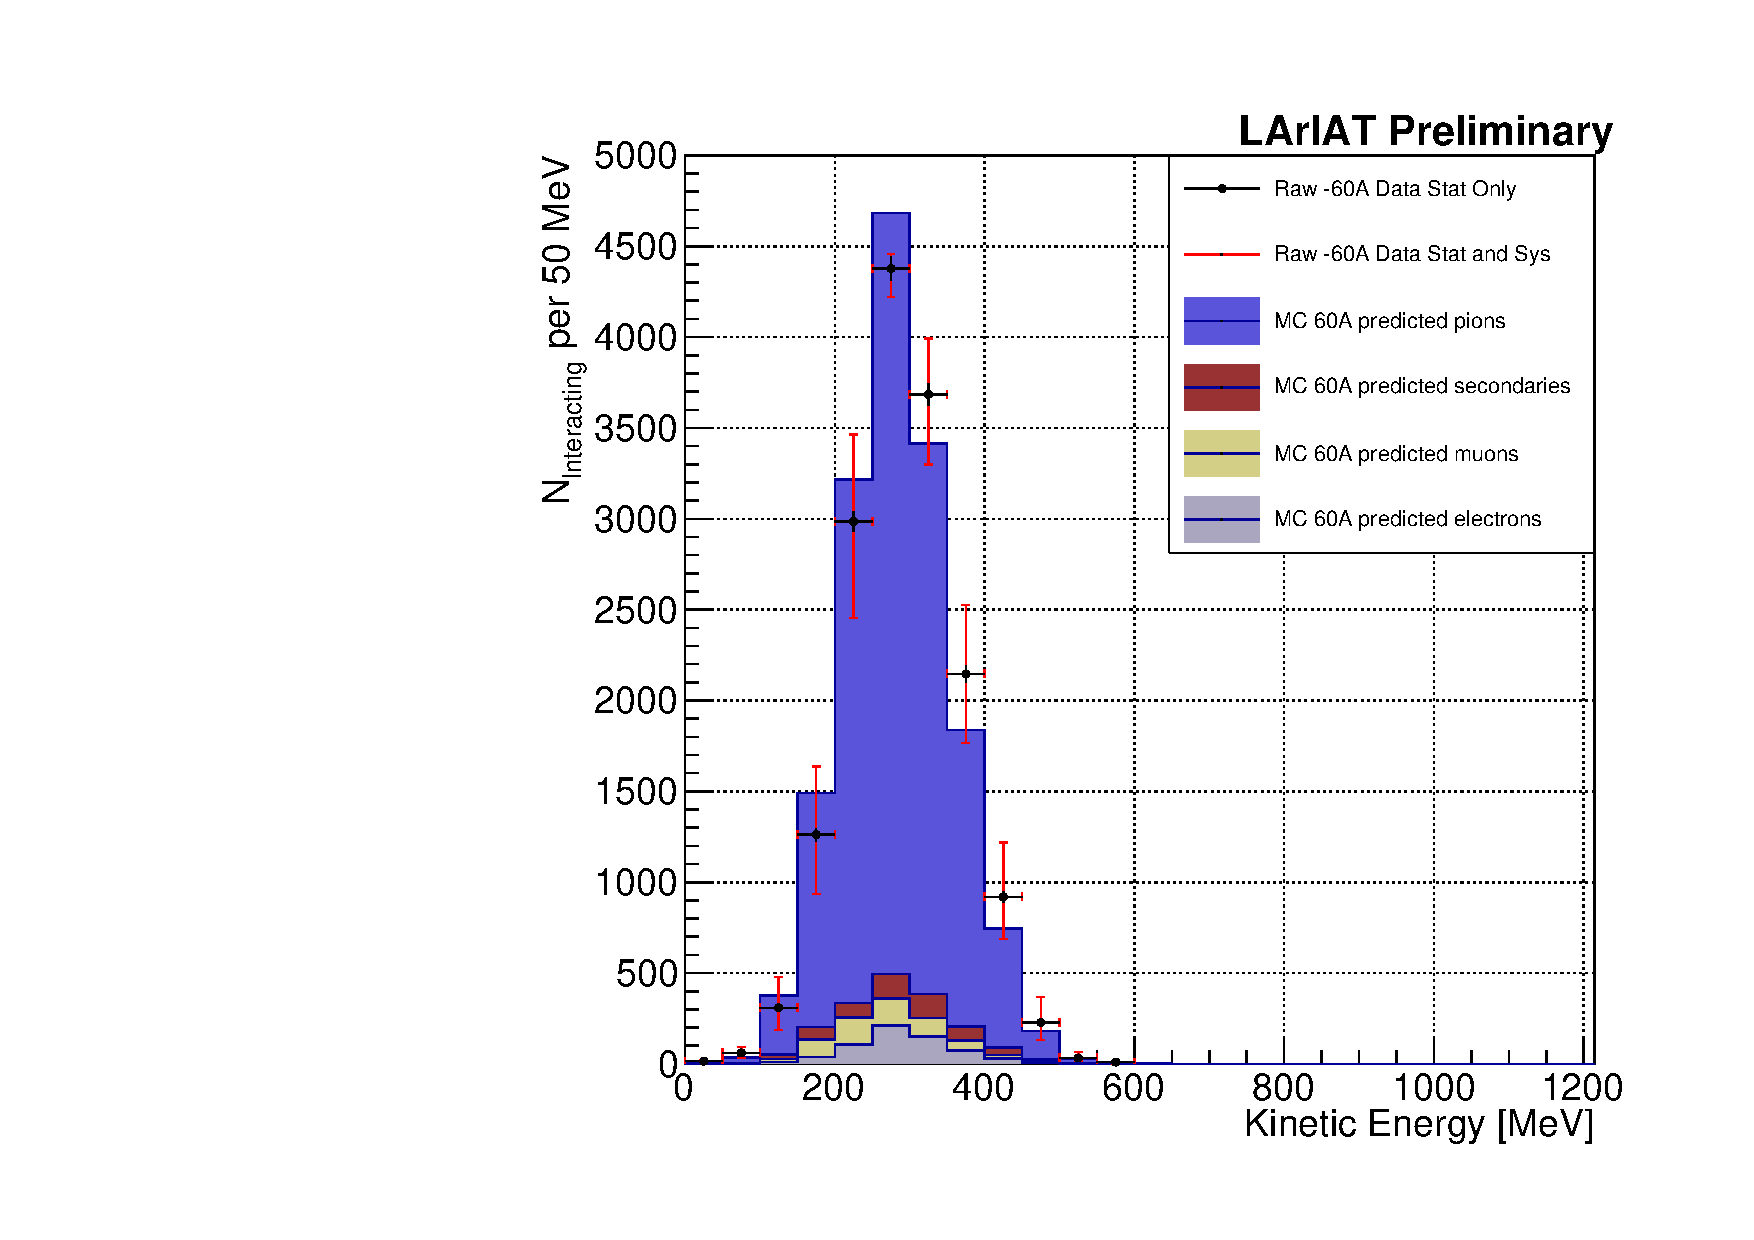
\includegraphics[width=0.48\textwidth]{Chapter-6/Images/Plots60A_MCData_Int_StatSyst.pdf}
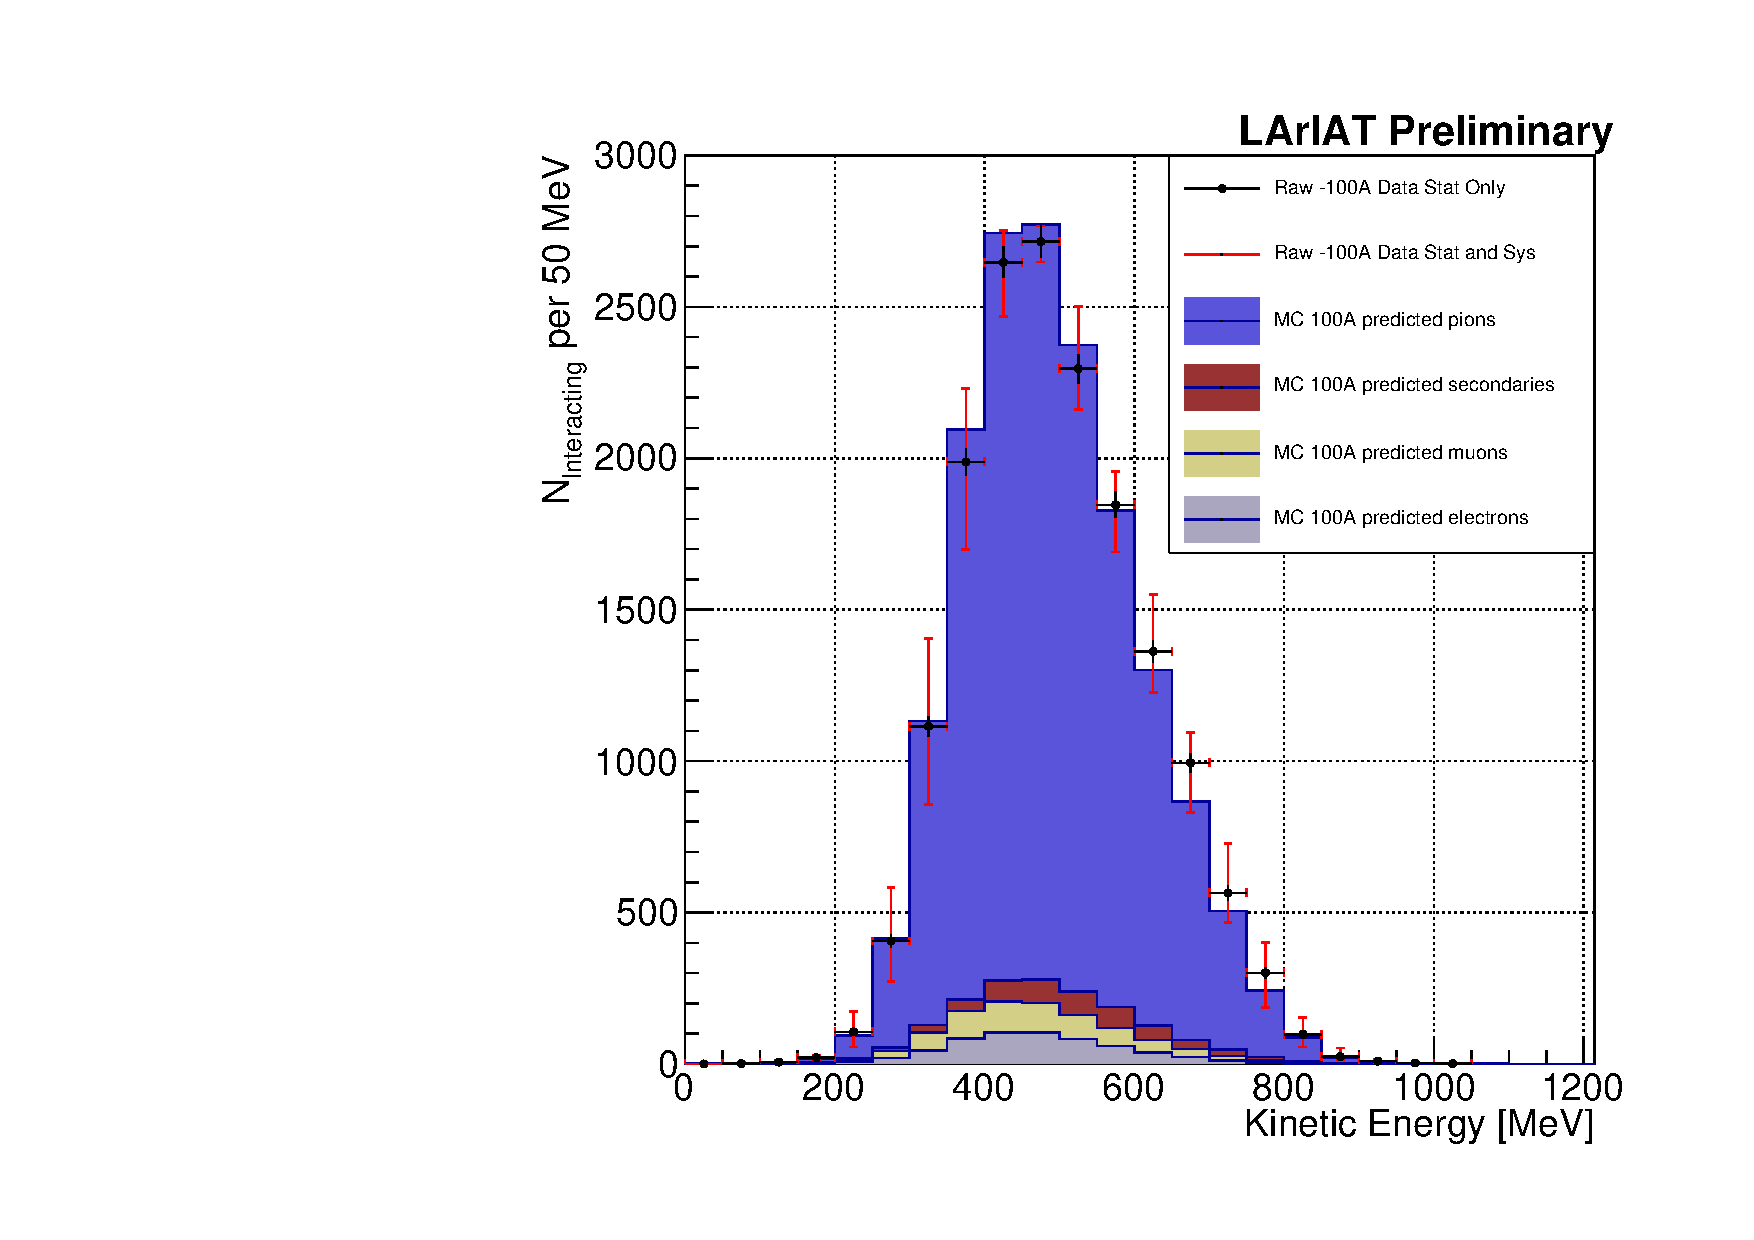
\includegraphics[width=0.48\textwidth]{Chapter-6/Images/Plots100A_MCData_Int_StatSyst.pdf}
\caption{Raw number of interacting pion candidates as a function of the reconstructed kinetic energy for the 60A runs (left) and for the 100A runs (right). The statistical uncertainties are shown in black, the systematic uncertainties in red.}
\label{fig:InteractingRaw}
\end{figure}


\begin{figure}
\centering  
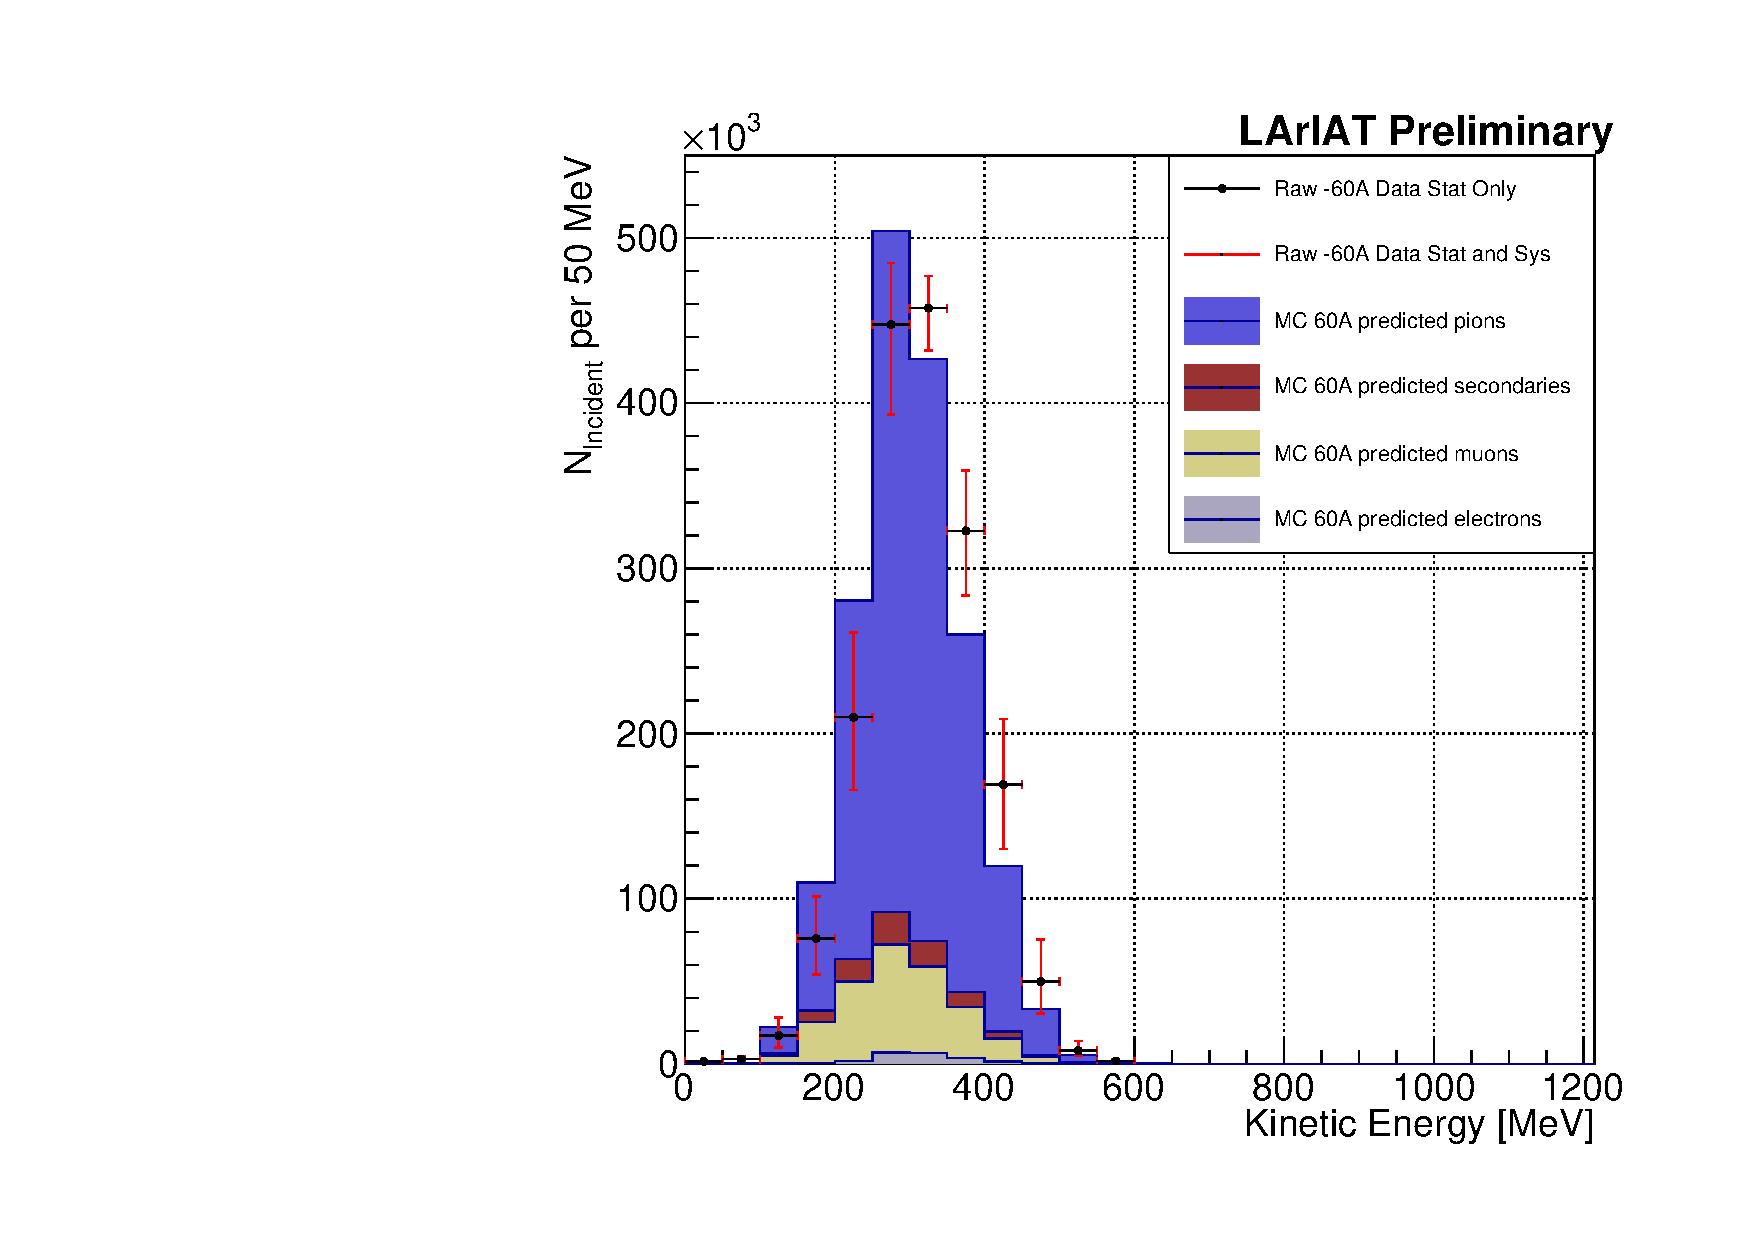
\includegraphics[width=0.48\textwidth]{Chapter-6/Images/Plots60A_MCData_Inc_StatSyst.pdf}
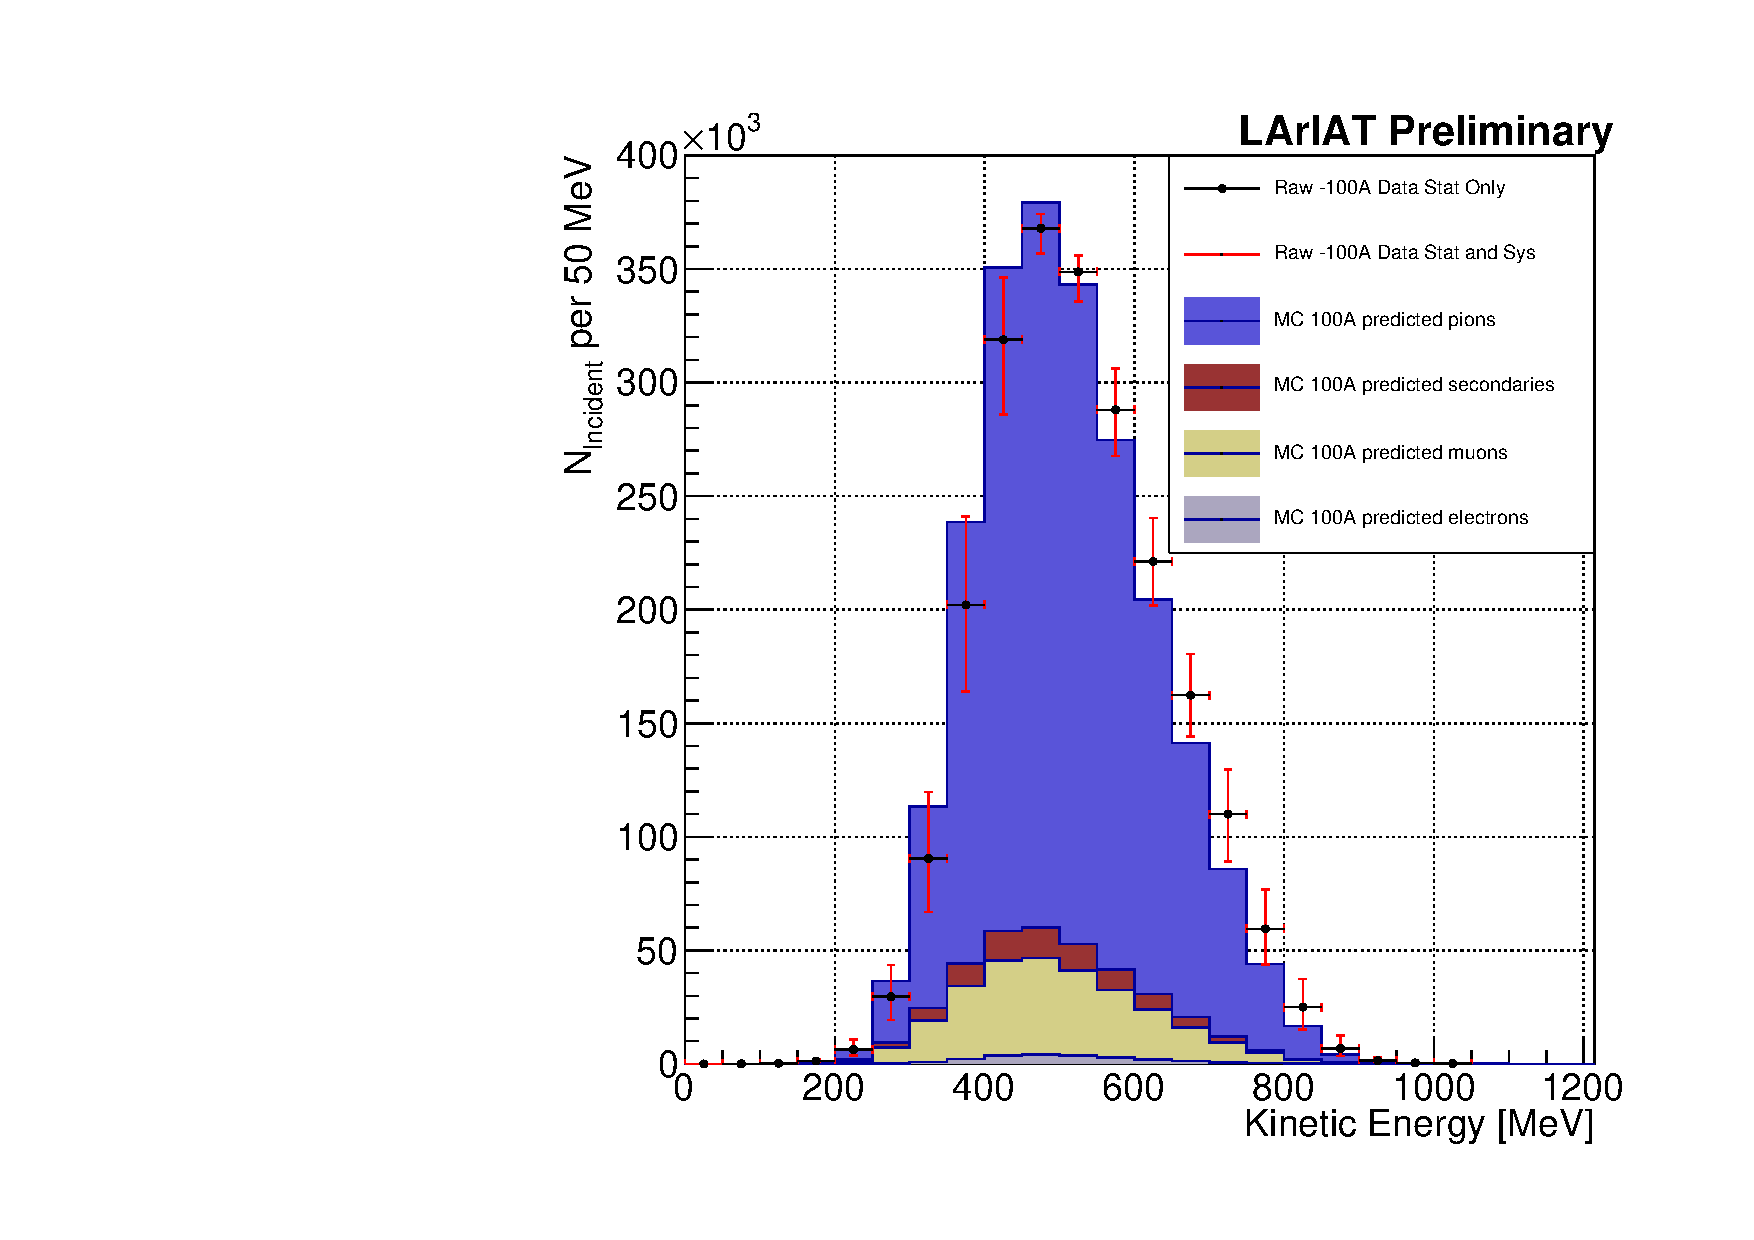
\includegraphics[width=0.48\textwidth]{Chapter-6/Images/Plots100A_MCData_Inc_StatSyst.pdf}
\caption{Raw number of incident pion candidates as a function of the reconstructed kinetic energy for the 60A runs (left) and for the 100A runs (right). The statistical uncertainty is shown in black, the systematic uncertainties in red.}
\label{fig:IncidentRaw}
\end{figure}

\begin{figure}
\centering  
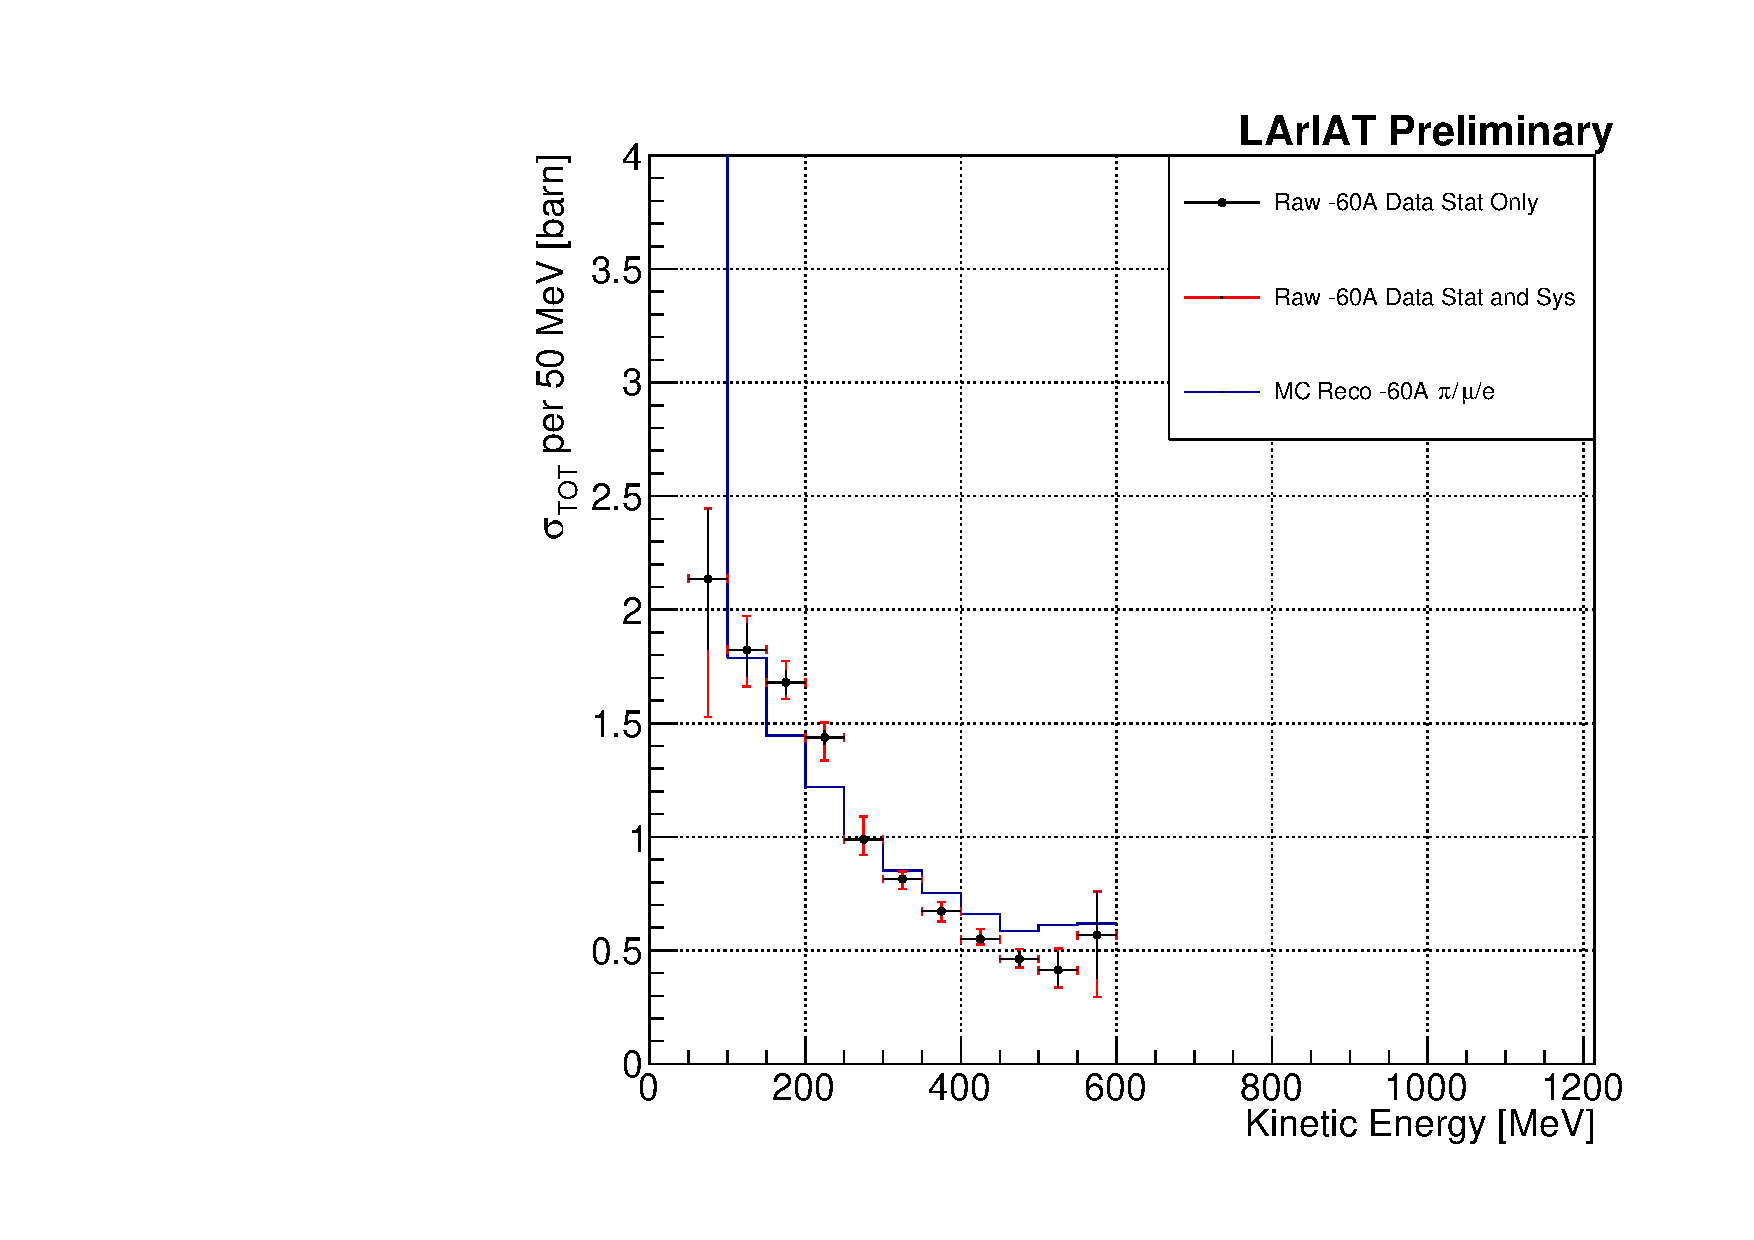
\includegraphics[width=0.48\textwidth]{Chapter-6/Images/Plots60A_MCData_XS_StatSyst.pdf}
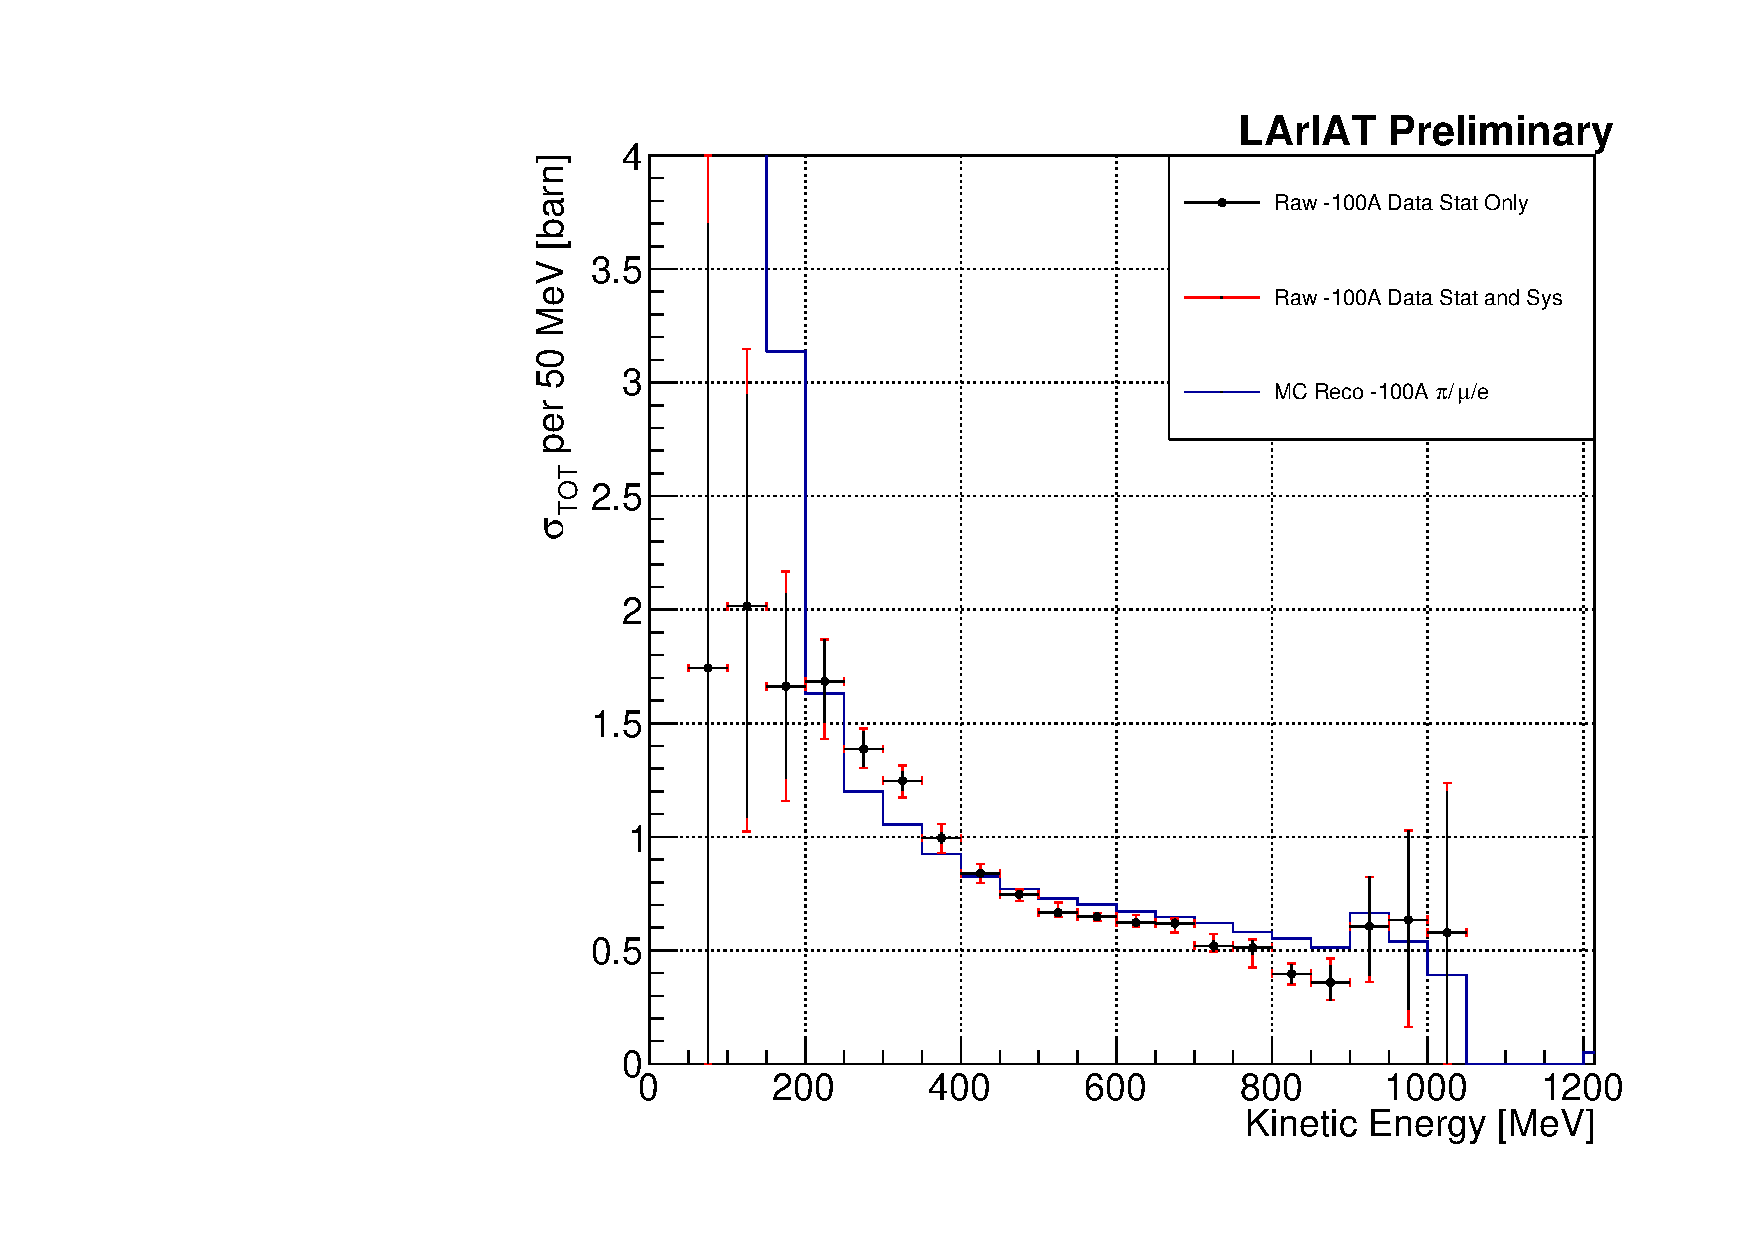
\includegraphics[width=0.48\textwidth]{Chapter-6/Images/Plots100A_MCData_XS_StatSyst.pdf}
\caption{Raw ($\pi^-$-Ar) total hadronic cross section for the 60A runs (left) and for the 100A runs (right). The statistical uncertainty is shown in black, the systematic uncertainties in red. The raw cross section obtained with a MC mixed sample of pions, muon and electrons in the percentage predicted by G4Beamline is shown in azure. }
\label{fig:XSRaw}
\end{figure}


\subsection{Statistical Uncertainty}\label{ch:StatUncertaintyXSRaw}
The statistical uncertainty for a given kinetic energy bin of the cross section  is calculated by error propagation from the statistical uncertainty on $N^{\text{TOT}}_{\text{Inc}}$ and $N^{\text{TOT}}_{\text{Int}}$ correspondent bin.  Since the number of incident particles in each energy bin is given by a simple counting, we assume that $N^{\text{TOT}}_{\text{Inc}}$ is distributed as a poissonian with mean and variance equal to $N^{\text{TOT}}_{\text{Inc}}$ in each bin.  
On the other hand, $N^{\text{TOT}}_{\text{Int}}$ follows a binomial distribution: a particle in a given energy bin might or might not interact.  The variance for the binomial is given by  
\begin{equation}
\text{\textsf{Var[}} N^{\text{TOT}}_{\text{Int}} \text{\textsf{]}}
 = \mathcal{N}P_{Interacting}(1-P_{Interacting}).
\label{eq:binVar}
\end{equation}

Since the interaction probability $P_{Interacting}$ is estimated by $\frac{ N^{\text{TOT}}_{\text{Int}}}{N^{\text{TOT}}_{\text{Inc}}}$ and the number of tries $\mathcal{N}$ is $N^{\text{TOT}}_{\text{Inc}}$, equation \ref{eq:binVar} translates into
\begin{equation}
\text{\textsf{Var[}} N^{\text{TOT}}_{\text{Int}} \text{\textsf{]}}
= N^{\text{TOT}}_{\text{Inc}}\frac{ N^{\text{TOT}}_{\text{Int}}}{N^{\text{TOT}}_{\text{Inc}}} (1-\frac{ N^{\text{TOT}}_{\text{Int}}}{N^{\text{TOT}}_{\text{Inc}}}) = N^{\text{TOT}}_{\text{Int}}(1-\frac{ N^{\text{TOT}}_{\text{Int}}}{N^{\text{TOT}}_{\text{Inc}}}). 
\end{equation}

$N^{\text{TOT}}_{\text{Inc}}$ and $N^{\text{TOT}}_{\text{Int}}$ are not independent. In fact, the population of a given bin for the interacting histogram always implies at least the population of the same bin in the incident histogram  (and possibly other incidents bins at higher energies). Thus, we conservatively calculate the statistical uncertainty on the cross section as 
\begin{equation}
\delta\sigma_{TOT}(E) = \sigma_{TOT}(E) \Big(\frac{\delta N^{\text{TOT}}_{\text{Int}}}{N^{\text{TOT}}_{\text{Int}}}+\frac{\delta N^{\text{TOT}}_{\text{Inc}}}{N^{\text{TOT}}_{\text{Inc}}}\Big) 
\end{equation}
where:
\begin{eqnarray}
\delta N^{\text{TOT}}_{\text{Inc}} = \sqrt[]{N^{\text{TOT}}_{\text{Inc}}} \\
\delta N^{\text{TOT}}_{\text{Int}} = \sqrt[]{N^{\text{TOT}}_{\text{Int}}\Big(1-\frac{ N^{\text{TOT}}_{\text{Int}}}{N^{\text{TOT}}_{\text{Inc}}}\Big)}.
\end{eqnarray}



\subsection{Treatment of Systematics} \label{ch:SysUncertaintyXSRaw}
The only systematic effect considered in the measurement of the raw cross section results from the propagation of the uncertainty associate with the measurement of the kinetic energy at each argon slab. As shown in Section \ref{ch:kinEn}, the uncertainty on the kinetic energy of a pion candidate at the j$^{th}$ slab of argon  is given by

\begin{eqnarray}
\delta KE_{j} &=& \sqrt{\delta p_{Beam}^2 + \delta E_{Loss}^2 +  \delta  E_{\text{dep FF-j}}^2}\\
&=& \sqrt{(2\% \text{ }p_{Beam})^2 +  ( 6 \text{ [MeV]})^2 +  (j-1)^2 (\sim0.08\text{ [MeV]})^2}.
\end{eqnarray}

We propagate this uncertainty  by varying the energy measurement $KE_{j}$ at each argon slab. We measure $N^{\text{TOT}}_{\text{Inc}}$,  $N^{\text{TOT}}_{\text{Int}}$ and the cross section  in three cases: first assigning the measured $KE_{j}$ at each kinetic energy sampling, then assigning $KE_{j} + \delta KE_{j}$, and finally assigning $KE_{j} - \delta KE_{j}$. The difference between the values obtained using the $KE_{j}$ sampling and the maximum and minimum values in each kinetic energy bin determines the systematic uncertainty.

%We propagate this uncertainty  by calculating the $N^{\text{TOT}}_{\text{Inc}}$,  $N^{\text{TOT}}_{\text{Int}}$ and cross section plots twice: first assigning $KE_{j} + \delta KE_{j}$ at each kinetic energy sampling, then assigning $KE_{j} - \delta KE_{j}$. The difference between the central value and the maximum and minimum value in each kinetic energy bin gives the systematic uncertainty.

\section{Corrections to the Raw Cross Section}\label{ch:PionXSCorrections}
As described in section \ref{ch:MCCorrections}, we need to apply a background correction and an efficiency correction in order to derive the pion cross section from the raw cross section.  The  cross section is given in equation \ref{eq:C}, 

\begin{equation}
   \sigma^{\pi^-}_{TOT}(E_{i})  = \frac{1}{n \text{ } \delta X}\frac{ \epsilon^{\text{Inc}}(E_i)  \hspace{0.2cm} C^{\pi MC}_{\text{Int}} (E_{i}) \hspace{0.2cm} N^{\text{TOT}}_{\text{Int}} (E_{i}) }{   \epsilon^{\text{Int}}(E_i) \hspace{0.2cm} C^{\pi MC}_{\text{Inc}} (E_{i}) \hspace{0.2cm}  N^{\text{TOT}}_{\text{Inc}} (E_{i})}.
 \tag{\ref{eq:C}}
\end{equation}

Section \ref{ch:BKGsubXSPuppa} describes the evaluation of pion content in the interacting and incident histograms, ($C^{\pi MC}_{\text{Int}} (E_{i})$  and  $C^{\pi MC}_{\text{Inc}} (E_{i})$) and the propagation to the cross section measurement of the relative systematic uncertainties.

Section \ref{ch:EFFXS} describes the procedure employed to obtain  the efficiency corrections $\epsilon^{\text{Int}}(E_i)$  and $\epsilon^{\text{Inc}}(E_i)$ and the propagation to the cross section measurement of the relative uncertainties.


\subsection{Background subtraction}\label{ch:BKGsubXSPuppa}
We use the procedure described in \ref{ch:PionXSBkgSub2} to evaluate the relative pion content in the interacting histogram $C^{\pi MC}_{\text{Int}} (E_{i})$  and the relative pion content in the incident $C^{\pi MC}_{\text{Inc}} (E_{i})$. We start by evaluating the relative pion content assuming the beamline composition simulated by G4Beamline, whose pion, muon and electron percentages per beam setting are reported again in the first line of Table \ref{tab:beamlineSys}. The left side of Figure \ref{fig:CorrectionsBeam} shows the  MC estimated  relative pion content for the interacting histogram as function of kinetic energy for the 60A runs (top) and 100A runs (bottom). The right side of the same figure shows the  MC estimated  relative pion content for the incident histogram as function of kinetic energy for the 60A runs (top) and 100A runs (bottom). In Figure \ref{fig:CorrectionsBeam} the central curves displayed in light blue are obtained using the beamline composition as predicted by G4Beamline: these are the correction curves for the relative pion content applied to data in equation \ref{eq:C}.

So, the question now becomes: how well do we know the beamline composition? In absence of additional data constraints,  we take a 100\% systematic uncertainty on the electron content, reported in lines 3 and 4 of Table \ref{tab:beamlineSys}. The effect of doubling or halving the electron percentage in the beam on the pion relative content is displayed in red in Figure \ref{fig:CorrectionsBeam}. We reserve a slightly different treatment for the muon content. Since G4Beamline tracks only particles which cross all the wire chambers, pion events that decay in flight from WC1 to WC4 are not recorded by G4Beamline. Pion decays in the beamline could  trigger the beamline detectors in data, if the produced muon propagates forward along the beamline. Thus, we take the G4Beamline prediction for muons as a lower bound in the composition: the effect of doubling the muon content (line 2 in Table \ref{tab:beamlineSys}) is shown in blue on Figure \ref{fig:CorrectionsBeam}. A future study of data from additional beamline detectors such as the Aerogel Chernkov detectors \cite{detectorPaper} or the muon range stack (see Section \ref{sec:MuRS}) has the potential of a narrowing the systematics uncertainty coming from the beamline compositon.


We propagate the uncertainty on the beamline composition  as a systematic uncertainty to the cross section by varying the beam composition for all the cases listed in Table \ref{tab:beamlineSys} and evaluating variation of obtained  data cross sections in each bin. This systematic uncertainty is summed in quadrature with the statistical uncertainty and the systematic uncertainty related to the kinetic energy measurement.


\begin{table}[p]
\centering
\begin{tabular}{| l | l | l | l | l | l | l | l | }
\hline
 &  \multicolumn{3}{|c|}{Magnet Current -60A} & \multicolumn{3}{|c|}{Magnet Current -100 A}\\

                                                  & MC $\pi^-$   & MC  $ \mu^-$ & MC  $e^-$ & MC  $\pi^-$ & MC  $\mu^-$ & MC  $e^-$  \\
\hline
Expected Composition          & 68.8	\%&4.6 \%&	26.6 \%&	87.4 \%&	3.7	\%&8.9 \% \\
Composition 2x Muons          & 64.2	\%&9.2 \%&	26.6 \%&	83.7 \%&	7.4	\%&8.9 \% \\
Composition 2x Electrons      &42.2	\%&4.6 \%&	53.2 \%&	78.5	\%&  3.7	\%&17.8 \%\\
Composition 0.5x Electrons   &82.1	\%&4.6 \%&	13.3 \%&	91.9 \%&	3.7	\%&4.4 \% \\
\hline
\end{tabular}
\caption{Beam composition variation for the study of systematics due to beam contamination.}
\label{tab:beamlineSys}
\end{table}

\begin{figure}[p]
\centering
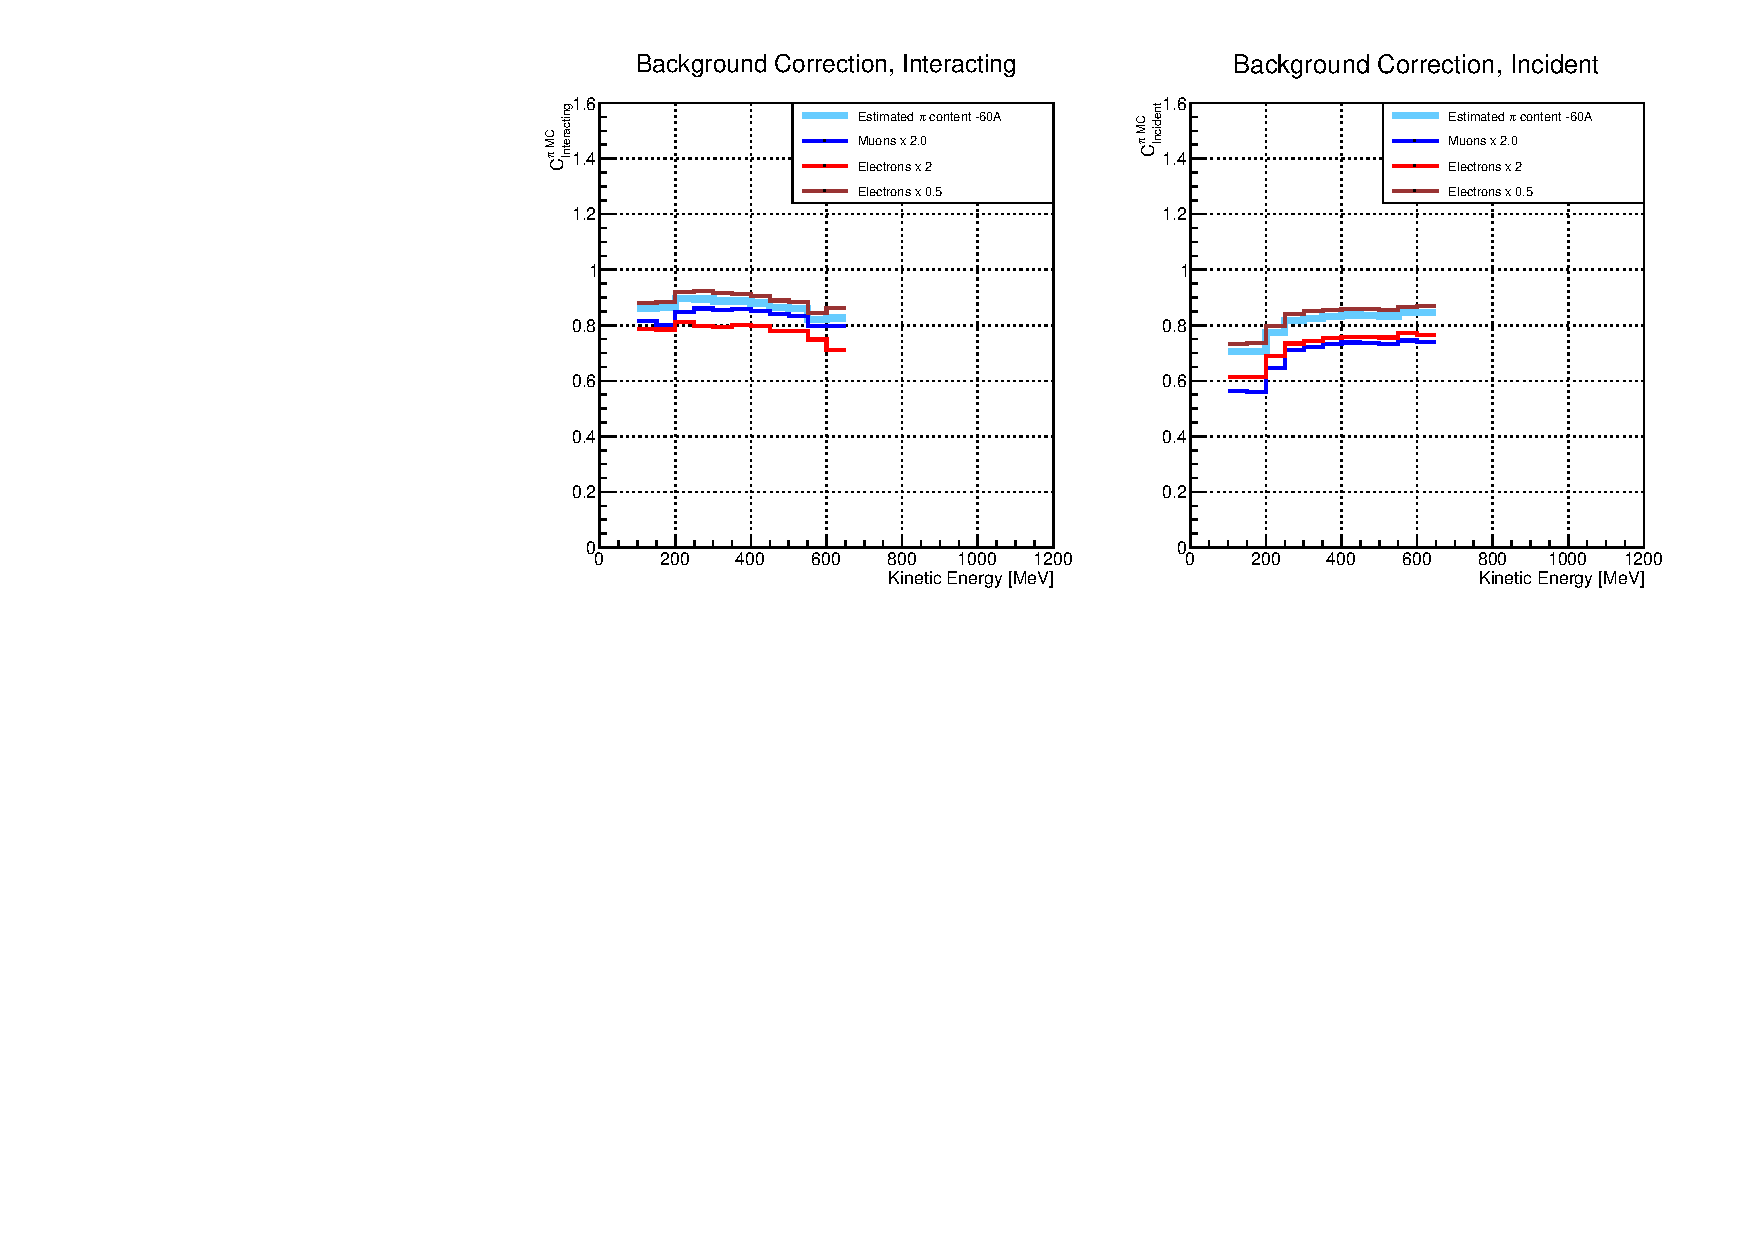
\includegraphics[width=\textwidth]{Chapter-6/Images/Bkg60A_inc_int.pdf}
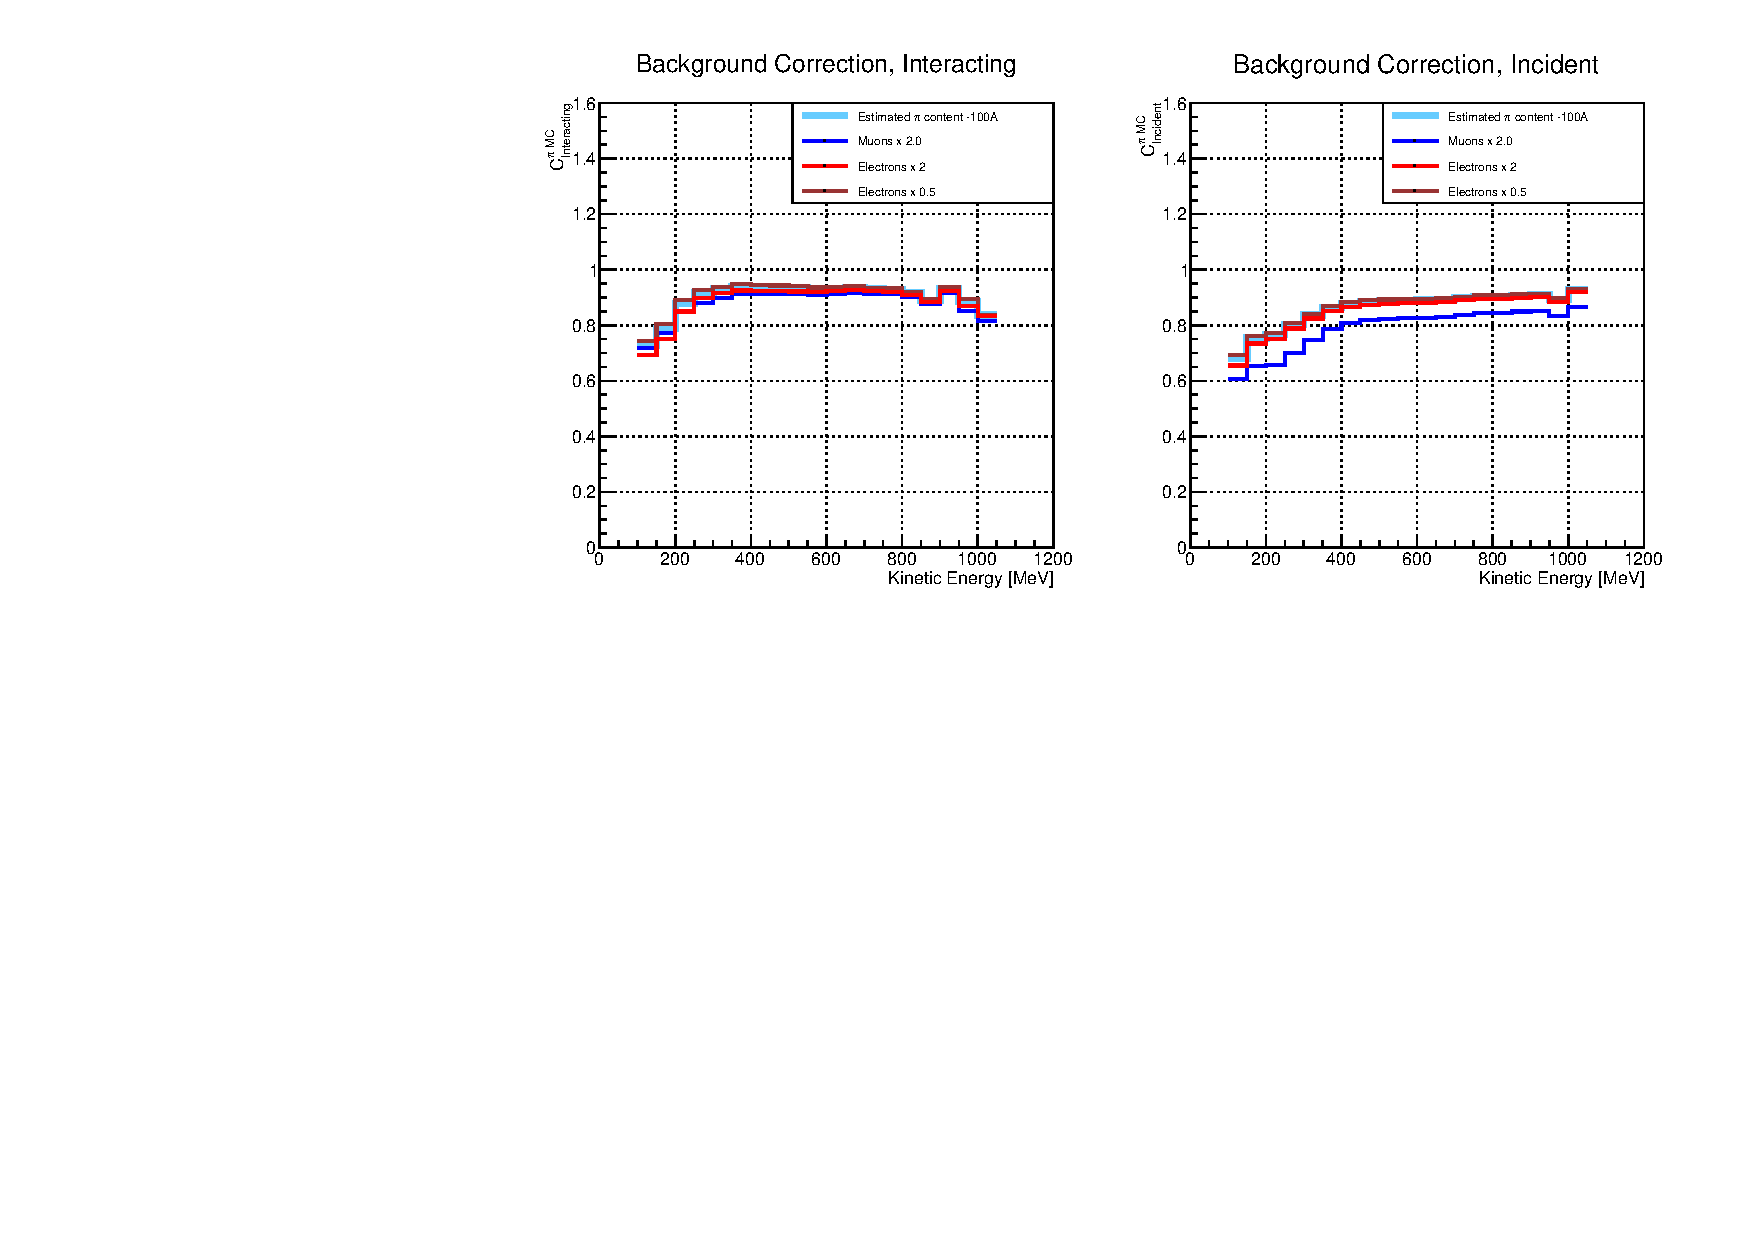
\includegraphics[width=\textwidth]{Chapter-6/Images/Bkg100A_inc_int.pdf}
\caption{\emph{Left:} MC estimated relative pion content for interacting histogram a function of kinetic energy for the 60A runs (top) and 100A runs (bottom), predicted background content in azure and muon and electron content variation in blue and red. \emph{Right:}  MC estimated relative pion content  for incident histogram a function of kinetic energy for the 60A runs (top)  and 100A (bottom), predicted background content in azure and muon and electron content variation in blue and red}
\label{fig:CorrectionsBeam}
\end{figure}



\subsection{Correction for Reconstruction Effects}\label{ch:EFFXS}
The interaction point for a particle in the selected sample for the total hadronic cross section analysis is the last point of its track that lies inside the LArTPC fiducial volume. This definition holds regardless the type of the interaction, i.e. if the TPC track ends within the fiducial volume, its last point will be the interaction point, no matter what the products of the interaction look like; on the other hand, if the track crosses the boundaries of the fiducial volume, the particle will be considered ``through going" and no interaction point will be found.  Given this definition, it is evident that we rely on the tracking algorithm to discern where the interaction occurred in the TPC  and correctly end the tracking. The tracking algorithm has an intrinsic angle resolution as shown in section \ref{sec:angleRes}, which limits its efficiency, especially in the case of elastic scattering occurring a low angles. \textcolor{red}{Plus, there are instance where INSERT HERE THE STUFF ABOUT THE MIGRATION}
Thus, we need to apply a correction accounting for mis-reconstruction of the interaction point in order to retrieve the true cross section.  This correction is evaluated separately for the interacting and incident histograms bin by bin, namely $\epsilon^{\text{int}}(E_i)$ and  $\epsilon^{\text{inc}}(E_i)$, and applied in the cross section formula as shown in  equation \ref{eq:C}. 

\subsubsection{Reconstruction Effects Correction: Procedure}\label{sec:EffCorrection}
We describe here the procedure to calculate the mis-reconstruction correction taking the interacting distribution as example and noting that the procedure is identical for the incident distribution. 

In section \ref{sec:angleRes}, we estimated the angular resolution for data and MC to be $\bar\alpha_{Data} = (5.0 \pm 4.5) \text{ deg}$  and 
$\bar\alpha_{MC} = (4.5 \pm 3.9) \text{ deg}$, respectively.  Most interaction angles smaller than the angular resolution will thus be indistinguishable  for the reconstruction. Thus, we claim we are able to  measure the cross section for interaction angles greater than 5.0 deg. Geant4 simulates interactions at all angles, as shown in figure \ref{fig:trueScatteringAngle}. In order to calculate the correction for reconstruction effects,  we select events which have an interaction angle greater than a given $\alpha_{res}$ to construct the true interacting and incident histograms (the denominator of the correction).

We derive the correction $\epsilon^{\text{int}}(E_i)$ on a set of pure pion MC, calculating its value bin by bin as the ratio between the true bin content and the correspondent reconstructed bin content. The true interacting distribution is obtained applying the thin slice method on true MC energy deposition up to the MC flagged true interaction point for interaction angles greater than 5$^\circ$. The reconstructed MC interacting distribution is obtained treating the MC events through the same reconstruction process as data: the interaction point is given by the end of the tracking and its energy is given by the reconstructed calorimetric information. The correction is then applied to in data bin by bin. In formulae, the correction is calculated to be

\begin{equation}
 \epsilon^{\text{Int}}(E_i)  =  \frac{N^{\text{ $\pi$ Reco MC}}_{\text{Interacting}} (E_{i})}{ N^{\text{ $\pi$ True MC}}_{\text{Interacting}} (E_{i})  },
\end{equation}
 
where $N^{\text{ $\pi$ True MC}}_{\text{Int}} (E_{i}) $ is the content of the $i$-th bin in the true interacting histogram, and $N^{\text{ $\pi$ Reco MC}}_{\text{Int}} (E_{i}) $ is the content of the $i$-th bin in the reconstructed interacting histogram. The correction is applied to data as follows

\begin{equation}
N^{\text{ $\pi$  Data}}_{\text{Int}} (E_{i})  =  \frac{N^{\text{$\pi$ Reco Data}}_{\text{Int}} (E_{i})}{\epsilon^{\text{Int}} (E_{i}) } = N^{\text{$\pi$ Reco Data}}_{\text{Int}} (E_{i}) \frac{N^{\text{ $\pi$ True MC}}_{\text{Int}} (E_{i})}{ N^{\text{ $\pi$ Reco MC}}_{\text{Int}} (E_{i})}.
\end{equation}

where $N^{\text{$\pi$ Reco Data}}_{\text{Int}} (E_{i})$ is the background subtracted bin content of the $i$-th bin in for the reconstructed interacting histogram for data, i.e. 
\begin{equation}
N^{\text{$\pi$ Reco Data}}_{\text{Int}} (E_{i}) =  N^{\text{TOT Data}}_{\text{Int}} (E_{i}) - B^{\text{Data}}_{\text{Int}} (E_i)  =  C^{\text{$\pi$ MC}}_{\text{Int}} (E_{i}) N^{\text{TOT Data}}_{\text{Int}} (E_{i}).
\end{equation}


 The systematics on this correction is estimated by varying the value of $\alpha_{res}$ between 0 deg and 4.5 deg and propagating the uncertainty on the cross section. 


Figure \ref{fig:EffCorr60A} shows $\epsilon^{\text{Int}}(E_{i})$ in the left side and $ \epsilon^{\text{Inc}}(E_i)$ on the right as a function of the kinetic energy for the 60A runs and their systematic uncertainty. Similarly, figure \ref{fig:EffCorr100A} shows $\epsilon^{\text{Int}}(E_{i})$ in the left side and $ \epsilon^{\text{Inc}}(E_i)$ on the right as a function of the kinetic energy for the 100A runs and their systematic uncertainty. 

\begin{figure}[p]
\centering
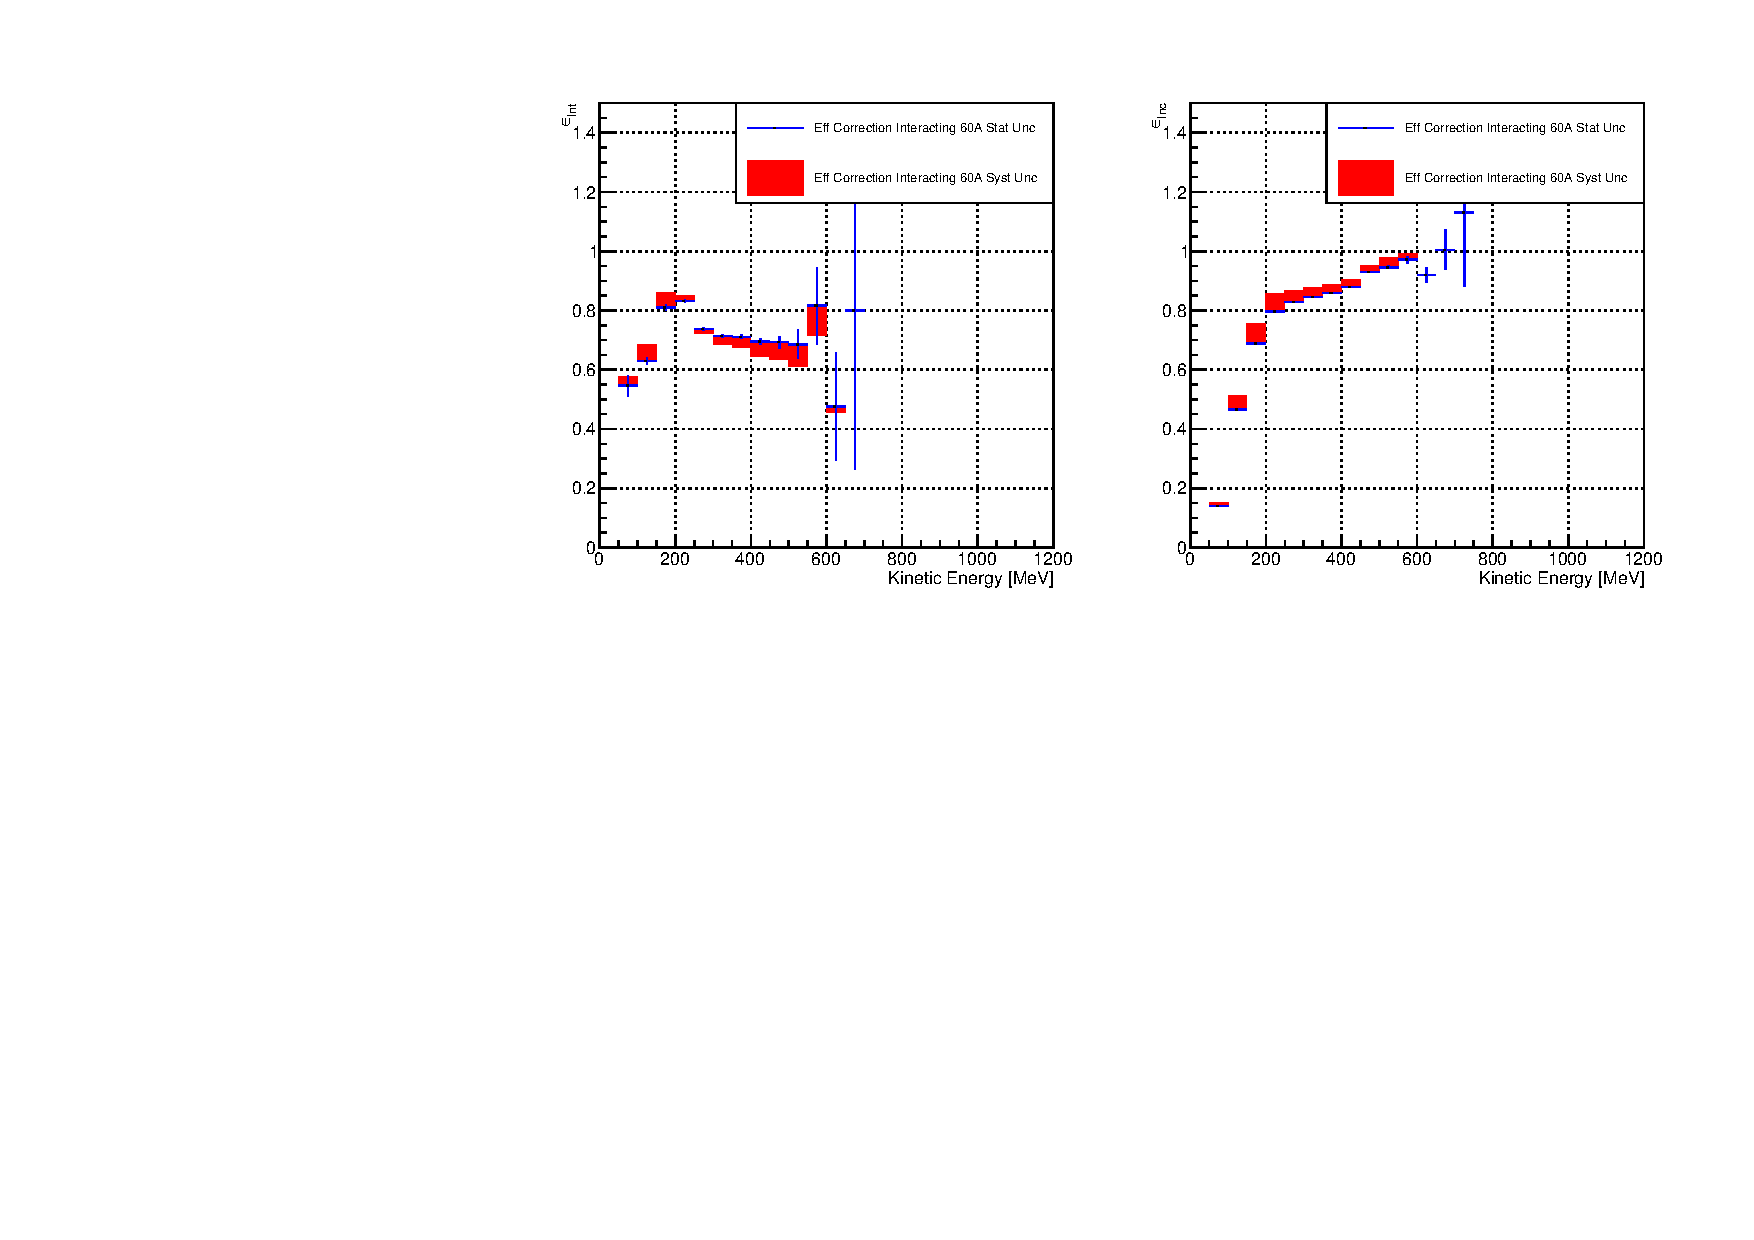
\includegraphics[width=\textwidth]{Chapter-6/Images/60AEffCorr.pdf}
\caption{\emph{Left:} Reconstruction effects correction on the 60A interacting histogram, statistical uncertainty in blue, systematic uncertainty in red. \emph{Right:}  Reconstruction effects correction on the 60A incident histogram, statistical uncertainty in blue, systematic uncertainty in red.}
\label{fig:EffCorr60A}
\end{figure}

\begin{figure}[p]
\centering
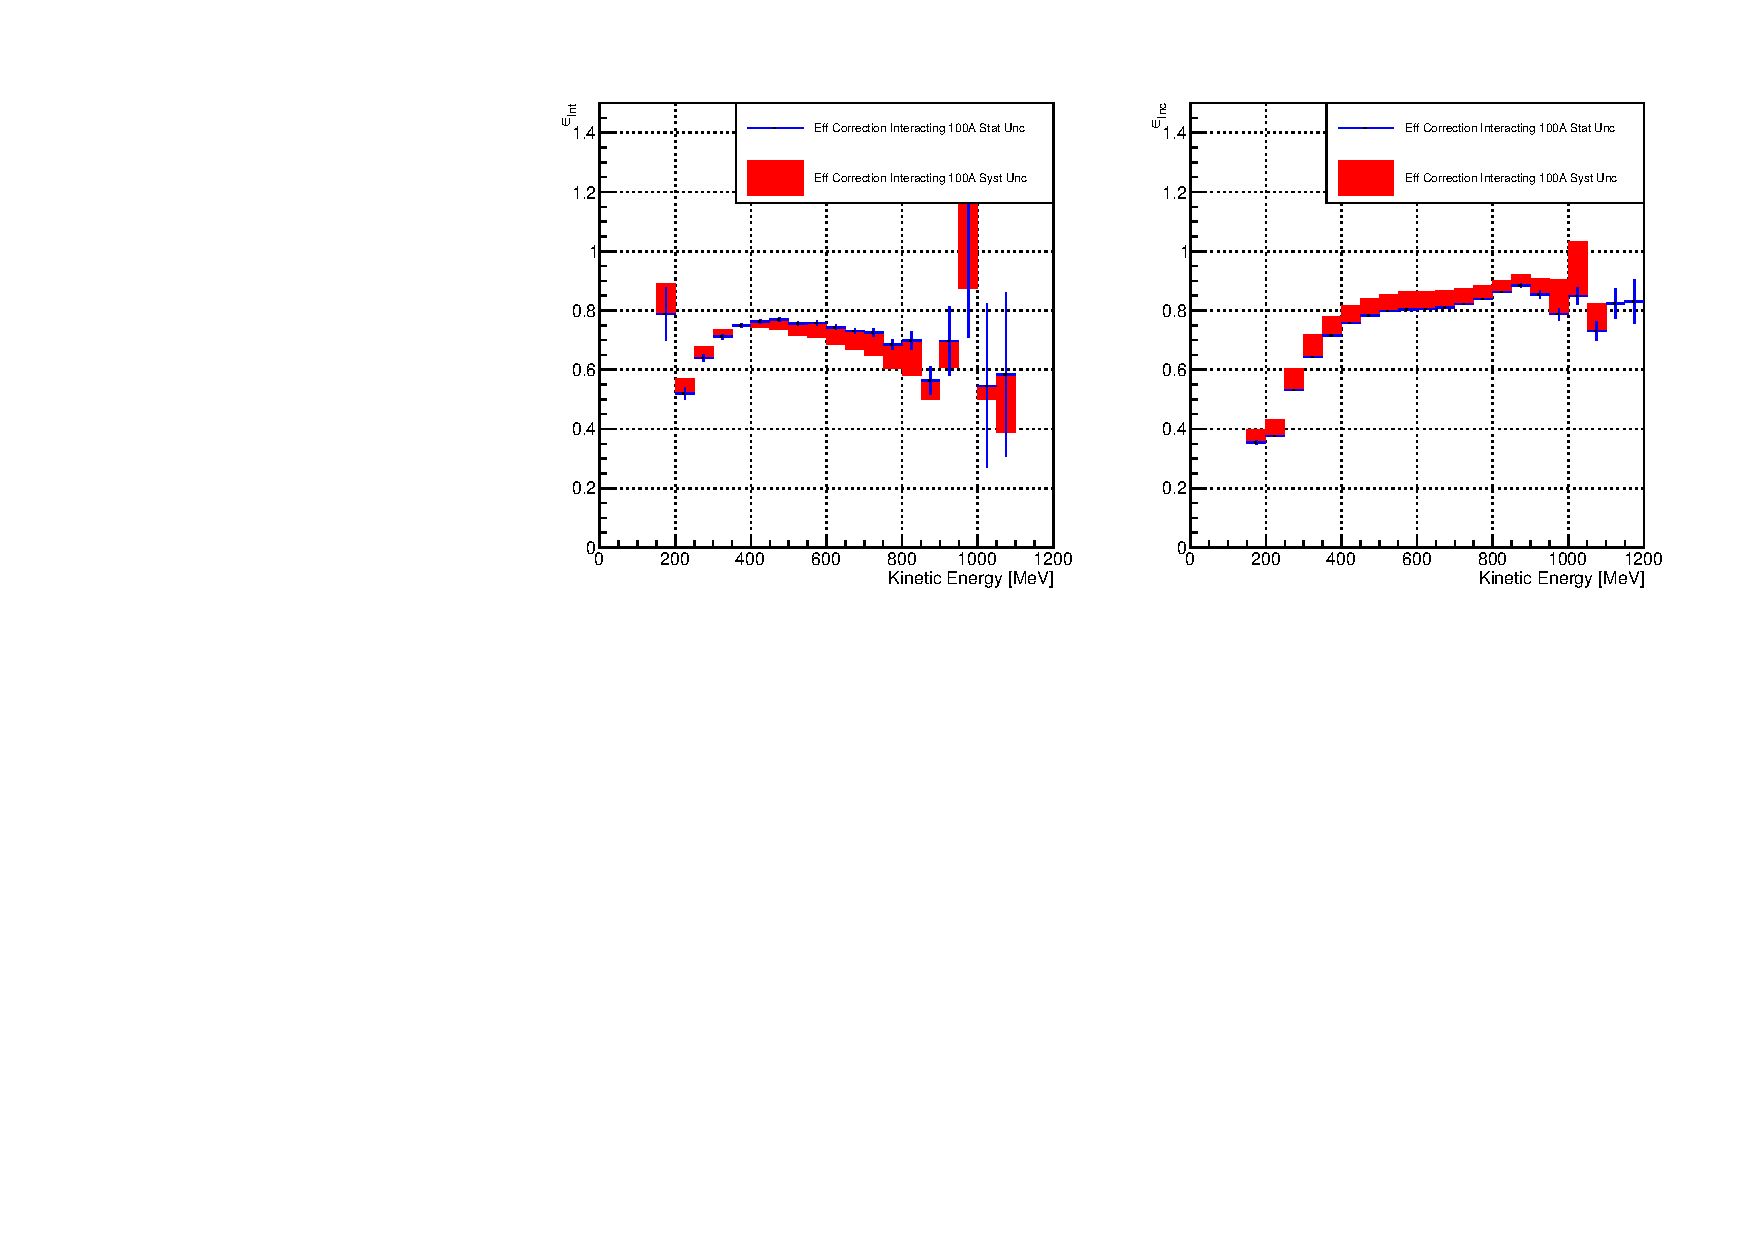
\includegraphics[width=\textwidth]{Chapter-6/Images/100AEffCorr.pdf}
\caption{\emph{Left:} Reconstruction effects correction on the 100A interacting histogram, statistical uncertainty in blue, systematic uncertainty in red. \emph{Right:}  Reconstruction effects correction on the 100A incident histogram, statistical uncertainty in blue, systematic uncertainty in red.}
\label{fig:EffCorr100A}
\end{figure}



\begin{figure}[p]
\centering
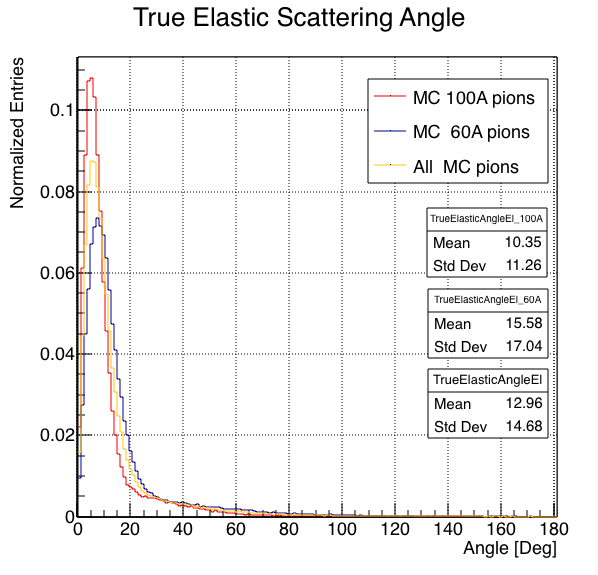
\includegraphics[width=0.48\textwidth]{Chapter-5/Images//cAngleTrue.png}
\caption{Distribution of the true scattering angle for a pion elastic scattering off the argon nucleus as simulated by Geant4.}
\label{fig:trueScatteringAngle}
\end{figure}




\clearpage
\section{Results}\label{ch:FinalPion}
Figure \ref{fig:FinalXSPion} shows the measurement of the ($\pi^-$-Ar) total hadronic cross section for  scattering angles greater than 5$^\circ$, as the result of the background subtraction and reconstruction effects correction to the raw cross section. The top left plot is the measurement obtained on the 60A data, statistical and systematic uncertainty shown in red. The top right plot is the measurement obtained on the 100A data, statistical uncertainty and systematic uncertainty shown in blue. The bottom plot shows the two measurements overlaid. In all three plot, the Geant4 prediction for the total hadronic cross section for angle scattering greater than 5$^\circ$ is displayed in green. 

The systematic uncertainty on the cross section is the sum in quadrature of the statistical uncertainty, the systematic uncertainty related to the kinetic energy measurement, the systematic uncertainty related to the beam composition and the systematic uncertainty related to the reconstruction effects correction.

The cross section measurements in the two datasets agree within the systematic uncertainty, even if the cross section measured in the 60A data is lower than the one measured in the 100A data in all overlapping bins except for the 200-250 MeV bin.

\begin{figure}[htb]
\centering
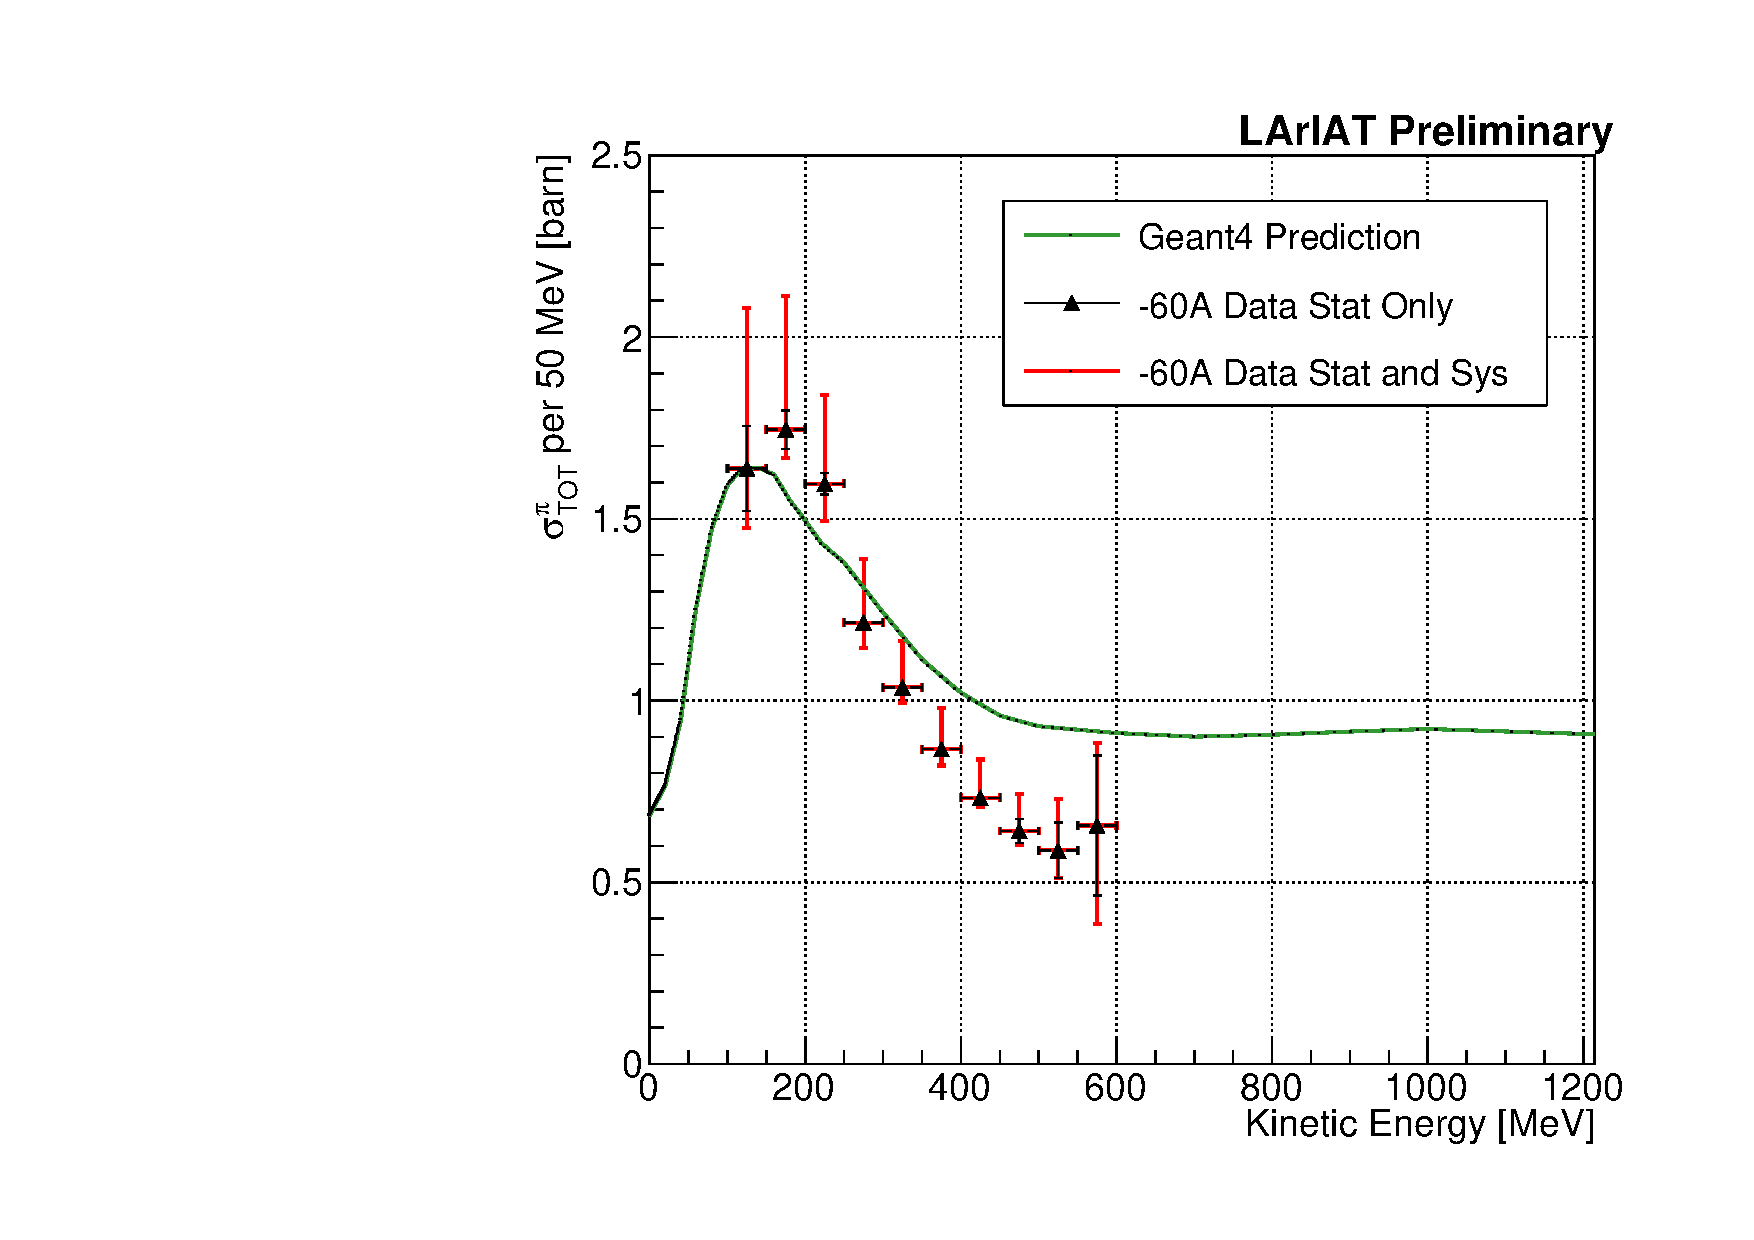
\includegraphics[width=0.48\textwidth]{Chapter-6/Images/TheMoneyPlot60A.pdf}
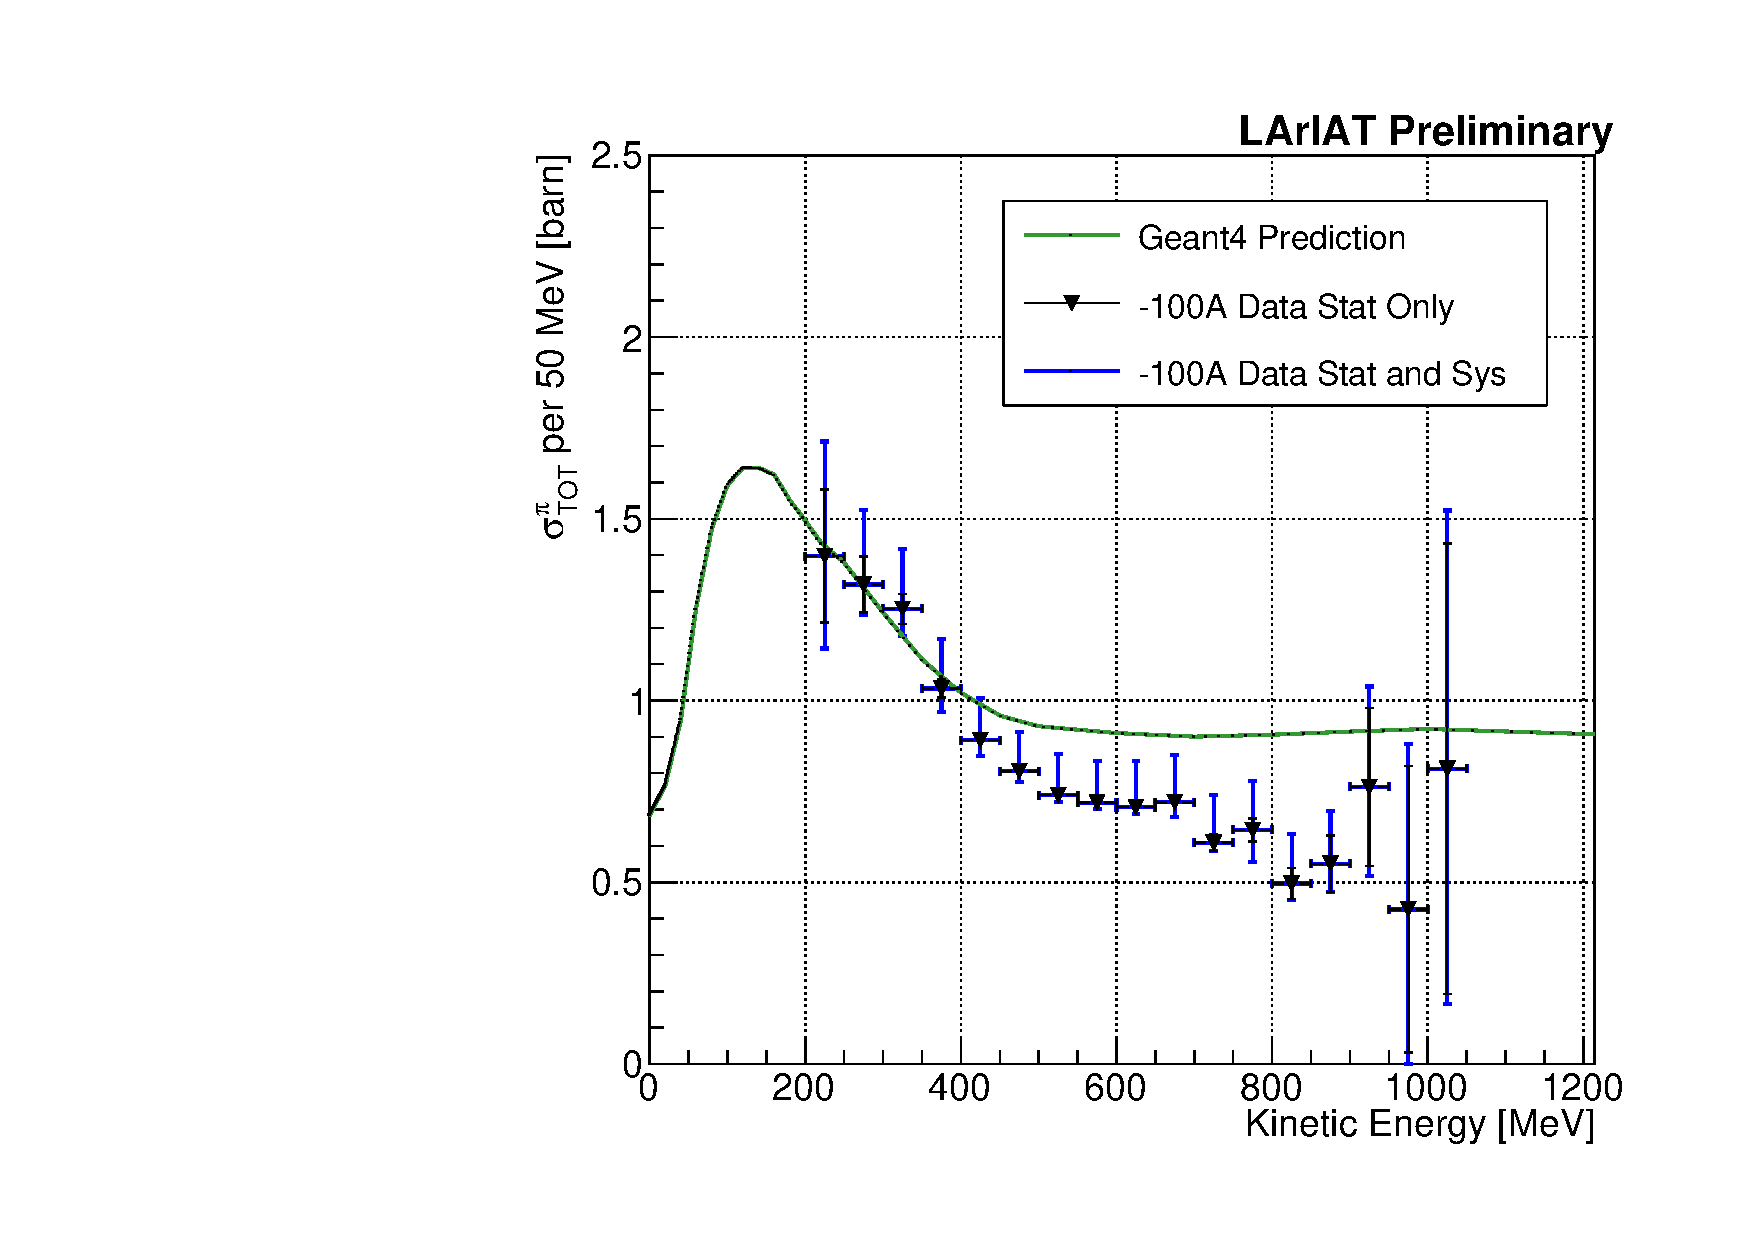
\includegraphics[width=0.48\textwidth]{Chapter-6/Images/TheMoneyPlot100A.pdf}
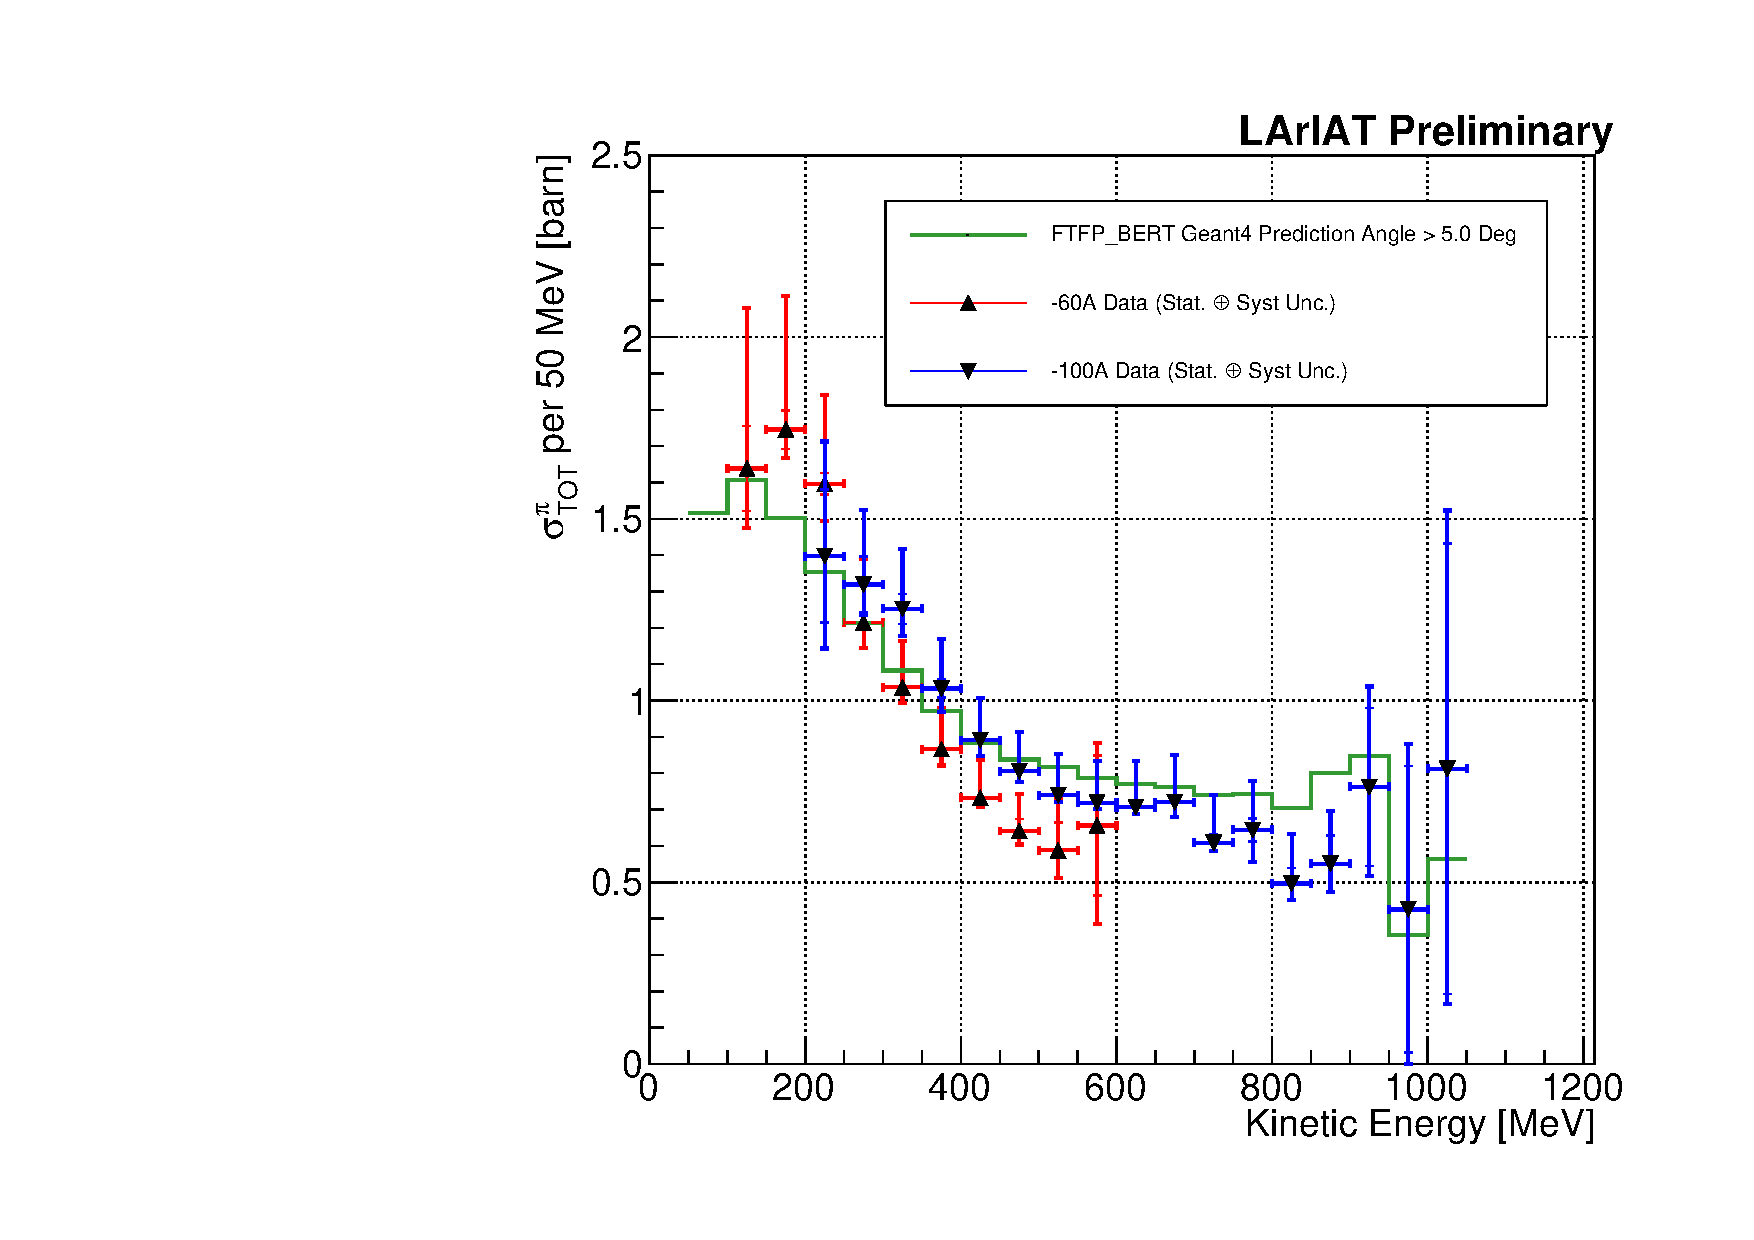
\includegraphics[width=0.48\textwidth]{Chapter-6/Images/TheMoneyPlot.pdf}
\caption{ \emph{Top Left:} ($\pi^-$-Ar) total hadronic cross section for  scattering angles greater than 5$^\circ$ measured in the 60A sample, statistical uncertainty in black and systematic uncertainty in red. The Geant4 prediction for the total hadronic cross section for angle scattering greater than 5$^\circ$ is displayed in green. \\ 
\emph{Top Right:} ($\pi^-$-Ar) total hadronic cross section for  scattering angles greater than 5$^\circ$ measured in the 100A sample, statistical uncertainty in black and systematic uncertainty in blue. The Geant4 prediction for the total hadronic cross section for angle scattering greater than 5$^\circ$ is displayed in green.\\
\emph{Bottom:} ($\pi^-$-Ar) total hadronic cross section measurements in the 60A and 100A samples overlaid with the  Geant4 prediction (green).}
\label{fig:FinalXSPion}
\end{figure}

The top panel of Figure \ref{fig:FinalXSResPion} shows the cross section obtained combining the two datasets. To combine the datasets, we merge the corrected interacting histogram for the 60A data with the interacting histogram for the 100A data; we apply the same merging with the incident histograms. We then calculate the cross section central point and statistical uncertainty using the merged interacting and incident histograms. The systematic uncertainty is calculated as the sum in quadrature of the original systematic uncertainties on the cross section measurements on the two separated data sets.

The bottom panel of figure  \ref{fig:FinalXSResPion} shows the relative difference between the measured cross section and the Geant4 predicted cross section.
A couple of considerations are in order here. On one hand, we note the general agreement between the measured and predicted cross sections. We expected the pion cross section in argon to be well modeled in Geant4, given the vast set of measurements available for pion interaction -- albeit not on argon. Thus, this agreement augments our confidence in the experimental methodology used.
On the other hand, this agreement is not perfect.  As a matter of fact, its imperfections are rather suggestive: we see a slight shift of the delta resonance at higher energies and a small shape difference, with a steeper drop between the delta region and the flatter part at energies greater than 400 MeV. 
Since we see room for improvement of the systematic uncertainties, we look forward to see if this difference in shape will be confirmed by further analyses.

\begin{figure}[htb]
\centering
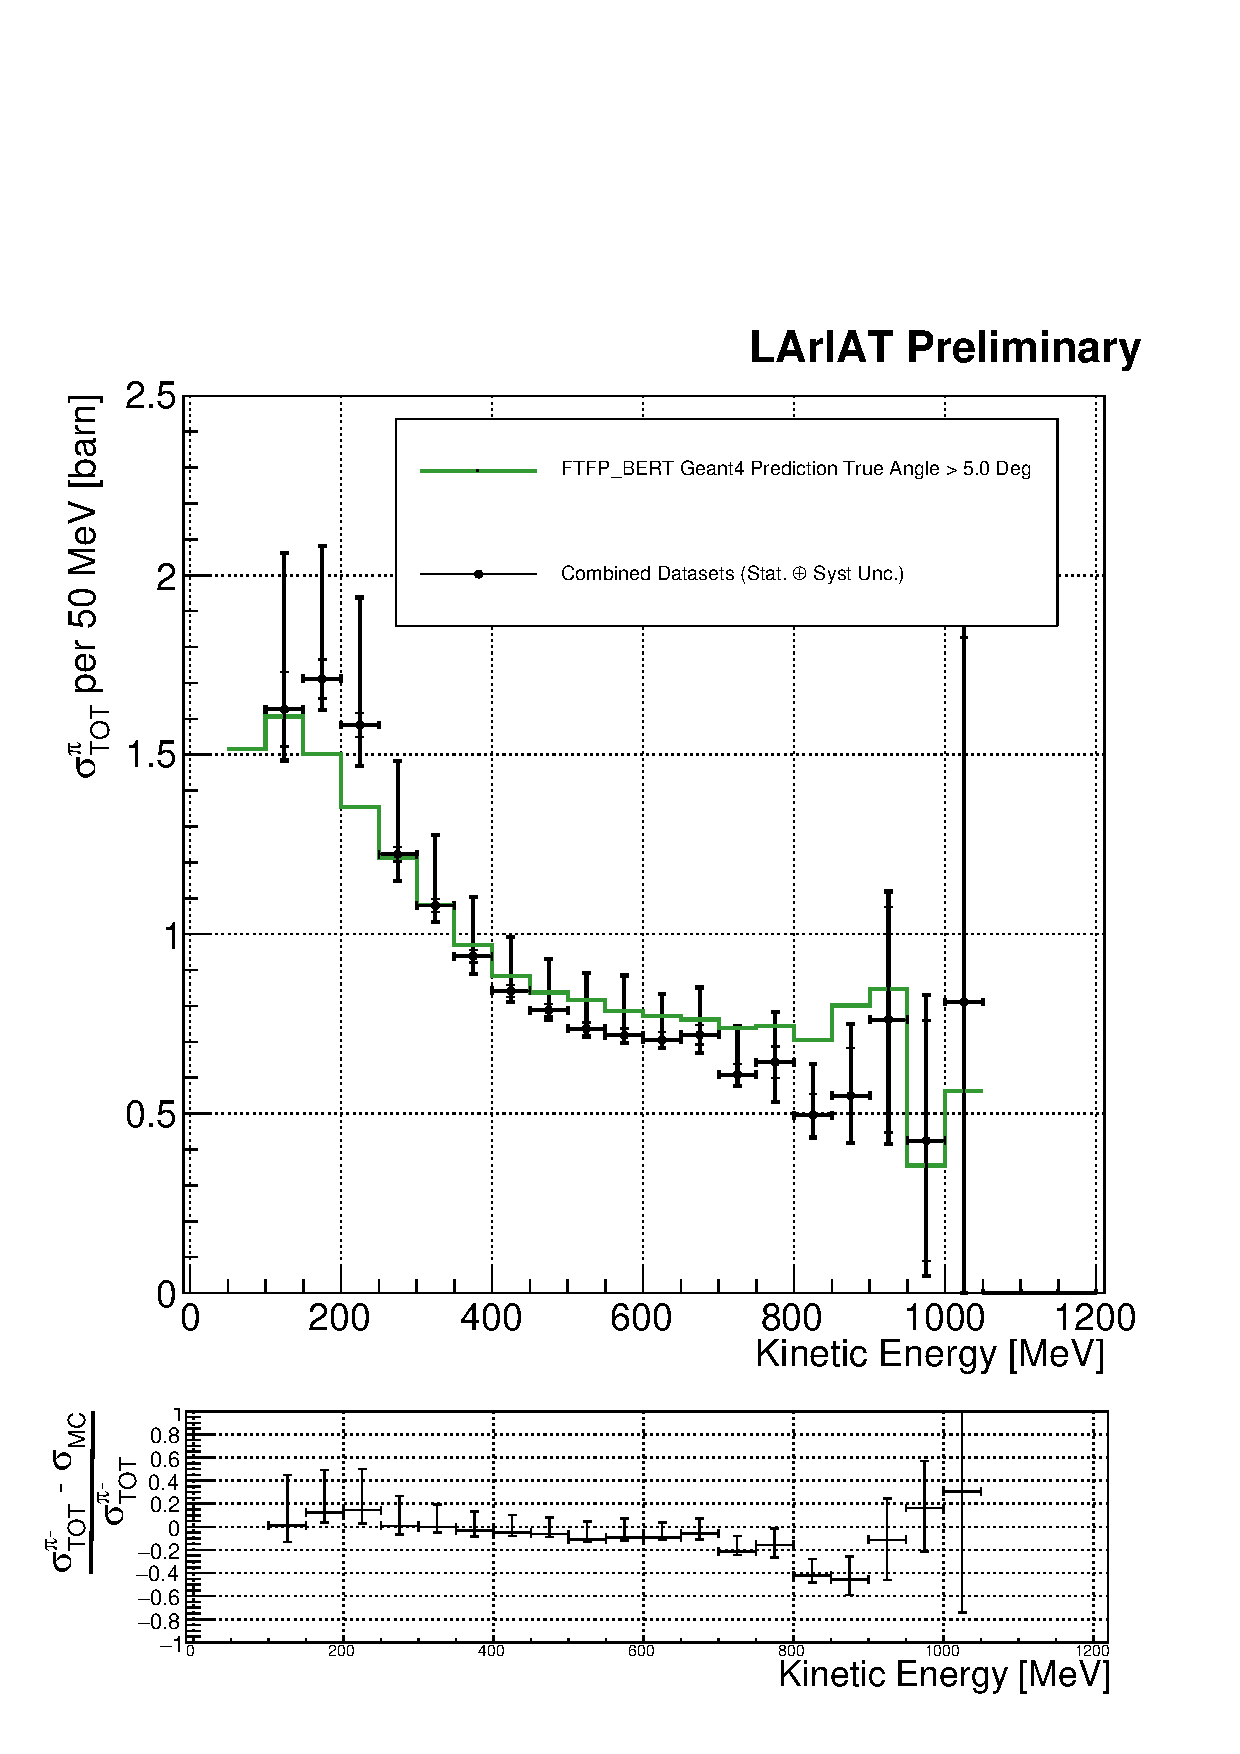
\includegraphics[width=\textwidth]{Chapter-6/Images/TheRealMoneyPlot.pdf}
\caption{ \emph{Top:} ($\pi^-$-Ar) total hadronic cross section for  scattering angles greater than 5$^\circ$ measured in the combined sample, statistical uncertainty and systematic uncertainty in black. The Geant4 prediction for the total hadronic cross section for angle scattering greater than 5$^\circ$ is displayed in green. \emph{Bottom:} Relative difference between the measured cross section and the Geant4 prediction. }
\label{fig:FinalXSResPion}
\end{figure}


%%%%%%%%%%%%%%%%%%%%%%%%%%%%%%%%%%%%%%%%%%%%%%%%%%%%%%%%%%%%%%%%%%%%%%
\begin{comment}
\subsection{Background subtraction}\label{ch:BKGsubXS}
%Even if pions are by far the biggest component of the beam in negative polarity runs, the LArIAT beam is not a pure pion beam. While useful to discriminate  pions/muons/electrons from kaons, and protons, the beamline detectors are not sensitive enough to  discriminate among the lighter particles in the beam: electrons, muons and pions fall under the same mass hypothesis. Thus, we need to assess the background from beamline particles other than pions in the event selections used for the pion cross section analysis and correct for its effects.

%\subsubsection{Beam Composition}\label{sec:BeamAtWC4}
%We define beamline background every TPC track matched to the WC track which is not a primary pion. Potentially, there are 4 different types of beamline background:
%\begin{itemize}
%\item[]1) electrons,
%\item[]2) muons,
%\item[]3) secondaries from pion events,
%\item[]4) matched pile up events.
%\end{itemize}

%The first step is to estimate what percentage of events used in the cross section calculation is not a primary pion.  The next two sections will illustrate this estimate for the electrons, muons and secondaries from pion event.
%We estimate the last type of background, the ``matched pile up" events, to be a negligible fraction, because of the definition of the WC2TPC match: we deem the probability of a single match with a halo particle in the absence of a beamline particle\footnote{ Events with multiple WC2TPC matches are always rejected.} negligibly small. \textcolor{red}{SHOW VTX distribution in WC2TPC match}


%\subsubsection{Background from Beamline Electrons and Muons}\label{stionEMu}
%\begin{figure}[b]
%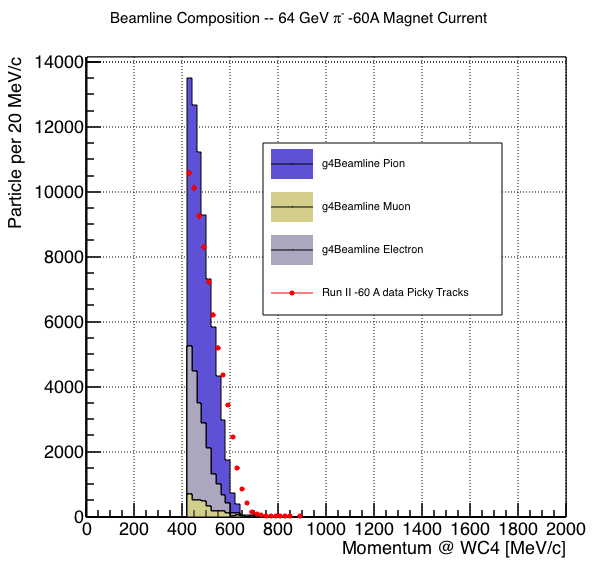
\includegraphics[width=0.5\textwidth,height=\textheight,keepaspectratio]{Studies/Figures//Beam60A.png}
%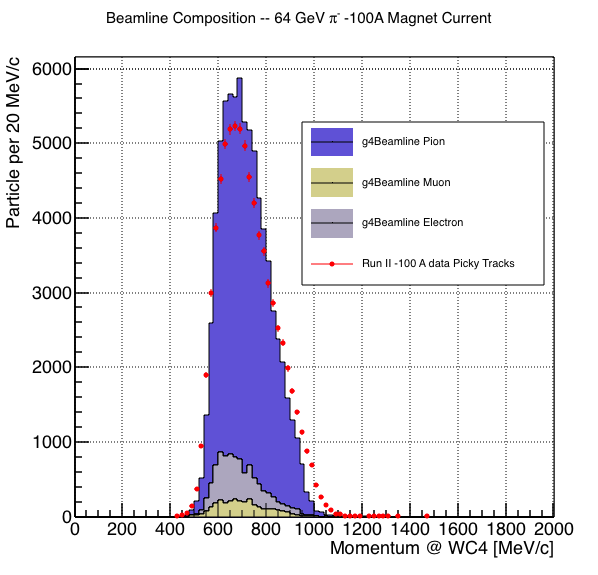
\includegraphics[width=0.5\textwidth,height=\textheight,keepaspectratio]{Studies/Figures//Beam100A.png}
%\caption{Beam composition for the -60A runs (left) and -100A runs (right). The solid blue plot represents the simulated pion content, the yellow plot represents the simulated muon content and the grey plot represents the simulated electron content. The plots are area normalized to the number of data events, shown in red. }
%\label{fig:BeamComposition}
%\end{figure}

%We estimate the percentage of electrons and muons in the beam via the G4Beamline MC. 
%Since the beamline composition is a function of the magnet settings, we simulate separately events for magnet current of -60A and -100A. 
%Table \ref{tab:beamline} shows the beam composition per magnet setting after the mass selection according to the G4Beamline simulation.
%\begin{table}[p]
%\centering
%\begin{tabular}{|l|c|c|}
%\hline
 %                   & I = -60 A           & I = -100 A \\ \hline
%G4Pions       &   68.8 \%           &      87.4 \%        \\ \hline
%G4Muons     &     4.6 \%           &        3.7 \%         \\ \hline
%G4Electrons &   26.6 \%           &        8.9 \%        \\ \hline
%\end{tabular}
%\caption{Simulated beamline composition per magnet settings}
%\label{tab:beamline}
%\end{table}


%Figure \ref{fig:BeamComposition} shows the momentum predictions from G4Beamline overlaid with data for the 60A runs (left) and for the 100A runs (right). The predictions for electrons, muons and pions have been staggered and their sum is area normalized to data, which is shown in red. Albeit not perfect, these plots show a reasonable agreement between the momentum shapes in data and MC. We attribute  the difference in shape to the lack of simulation of the WC efficiency in the MC which is momentum dependent and leads to enhance the number events in the center of the momentum distribution.

%Once the beam composition at WC4 is know,  we simulate the electrons, muons and pions with the DDMC and we subject the three samples to the same selection chain (WC2TPC match, shower filter, pile up filter). The percentage of electrons and muons surviving the selection chain weighted by the beam composition is the  electron and muon background in the pion cross section sample, as shown in Table \ref{tab:MCafterCutContaminants}.

%\subsubsection{Background from secondaries at TPC Front Face}
%Pions can travel the length of the LArIAT beamline and interact hadronically in the steel or in the non-instrumented argon upstream to the TPC front face. Or, they could decay in flight between WC4 and the TPC. One of the interaction products can leak into the TPC and be matched with the WC track, contributing to the pool of events used for the cross section calculation. We call this type of particles ``secondaries" from pion events, with a terminology inspired by Geant4. 
%We estimate the number of secondaries using the DDMC pion sample.  The percentage of secondaries is given by the number of matched WC2TPC tracks whose corresponding particle is not flagged as primary by Geant4.  The secondary to pion ratio is 4.9\% in the 60A sample and $Y$\% in the 100A sample.

\subsection{Background Contribution to the Cross Section}\label{sec:Correction}



\subsubsection{Treatment of Systematics}


\end{comment}

